\documentclass[aspectratio=169, dvipdfmx, 11pt]{beamer}
\usepackage{here, amsmath, latexsym, amssymb, bm, ascmac, mathtools, multicol, tcolorbox, subfig}
\usetheme{metropolis}           % Use metropolis theme
\setbeamercolor{background canvas}{bg=white}
\setbeamercolor{block title}{bg=white}
% Mathematical Sets
\newcommand{\NaturalNumberSet}{\mathbb{N}}
\newcommand{\RealNumberSet}{\mathbb{R}}
\newcommand{\NDemenstionalRealEuclideanSpace}{\mathbb{R}^n}
\newcommand{\NDemenstionalRealSymmetricMatrixSpace}{\mathbb{S}^n}

% Symbols like prefix
\newcommand{\Closure}[1]{\text{\rm cl\:${#1}$}} % cl
\newcommand{\Domain}[1]{\text{\rm dom\:${#1}$}} % dom
\newcommand{\Epigraph}[1]{\text{\rm epi\:${#1}$}} % epi
\newcommand{\Trace}[1]{\text{\rm tr$({#1})$}} % tr
\newcommand{\InnerProduct}[2]{\left\langle {#1},{#2}\right\rangle} % <x,y>

% Extended real valued function e.g. f: X -> Rv{+∞}
% #1: function symbol
% #2: domain of function
\newcommand{\ExtendedRealValuedFunction}[2]{{#1}: {#2} \to \RealNumberSet \cup \{+\infty\}}

% Conjugate function e.g. f*
% #1: function symbol
\newcommand{\ConjugateFunction}[1]{{#1}^*}

% (Useful) Texts
\newcommand{\SuchThat}{\:\text{s.t.}\:}

% Set form e.g. {x | ...}
% #1: element
% #2: conditions
\newcommand{\SetForm}[2]{
  \{{#1}\:|\:{#2}\}
}

\title[Asymptotic Function の半正定値計画問題への応用]{Applications of Asymptotic Function to Semidefinite Programming}
\subtitle{漸近関数の半正定値計画問題への応用}
\author[Ryota Iwamoto]{F22A034C 岩本 崚汰}
\institute[Niigata Univ]{Niigata Univ}
\date{9th, February, 2024}
\begin{document}
\maketitle

\begin{frame}{Contents}
  \tableofcontents
\end{frame}

% 1. Motivation
% ----------------------------------------------------------------
\section{Introduction \& Motivation}

% 1.1 Motivation

\begin{frame}{Introduction \& Motivation}
  Consider the following general \textbf{composite} optimization problem:

  \begin{equation}
    \begin{aligned}
      \inf \:& \phi(x) \\
      \text{s.t.} \:& x \in \NDemenstionalRealEuclideanSpace
    \end{aligned} \tag{CM} \label{eq:cm}
  \end{equation}

  with

  \begin{equation}
    \phi(x)=
    \begin{cases}
      f_0 (x) + H_{\infty} (f_1(x), \ldots, f_m(x)) & \text{if $x \in \bigcap_{i =1}^{m} \Domain{f_i}$,} \\
      +\infty      & \text{otherwise,} \notag
    \end{cases}
  \end{equation}

  where $f_0, \ldots, f_m$ are real-valued proper l.s.c. functions, $H$ is a proper convex l.s.c. function, and $H_{\infty}$ is the asymptotic function of $H$.
\end{frame}

\begin{frame}{Introduction \& Motivation}
  Consider the approximate problem for the problem \eqref{eq:cm}:

  \begin{equation}
    \begin{aligned}
      \inf \:& \phi_r(x) \\
      \text{s.t.} \:& x \in \NDemenstionalRealEuclideanSpace
    \end{aligned} \tag{CMr} \label{eq:cmr}
  \end{equation}
  with
  \begin{equation}
    \phi_r(x)=
    \begin{cases}
      f_0 (x) + H_r (f_1(x), \ldots, f_m(x)) & \text{if $x \in \bigcap_{i =1}^{m} \Domain{f_i}$,} \\
      +\infty      & \text{otherwise,} \notag
    \end{cases}
  \end{equation}

  \begin{alertblock}{Remark}
    The asymptotic function $H_\infty$ of a given proper l.s.c. convex function $H$ can be approximated by
    \begin{equation}
      H_{\infty}(y) = \lim_{r \to 0^+} H_r(y) \coloneqq  rH(\frac{y}{r}), \forall y \in \Domain{H}. \notag
    \end{equation}
  \end{alertblock}
\end{frame}

\begin{frame}{Motivation}
In the $n$-dimensional real Euclidean space $\NDemenstionalRealEuclideanSpace$, asymptotic cones and functions play a significant role to consider optimization problems. In addition, semidefinite programming (SDP) is one of the most important optimization problems because these problems have appeared in various area of mathematical sciences. The following content explains the relation between asymptotic cones and SDP.
\bigskip

\centering
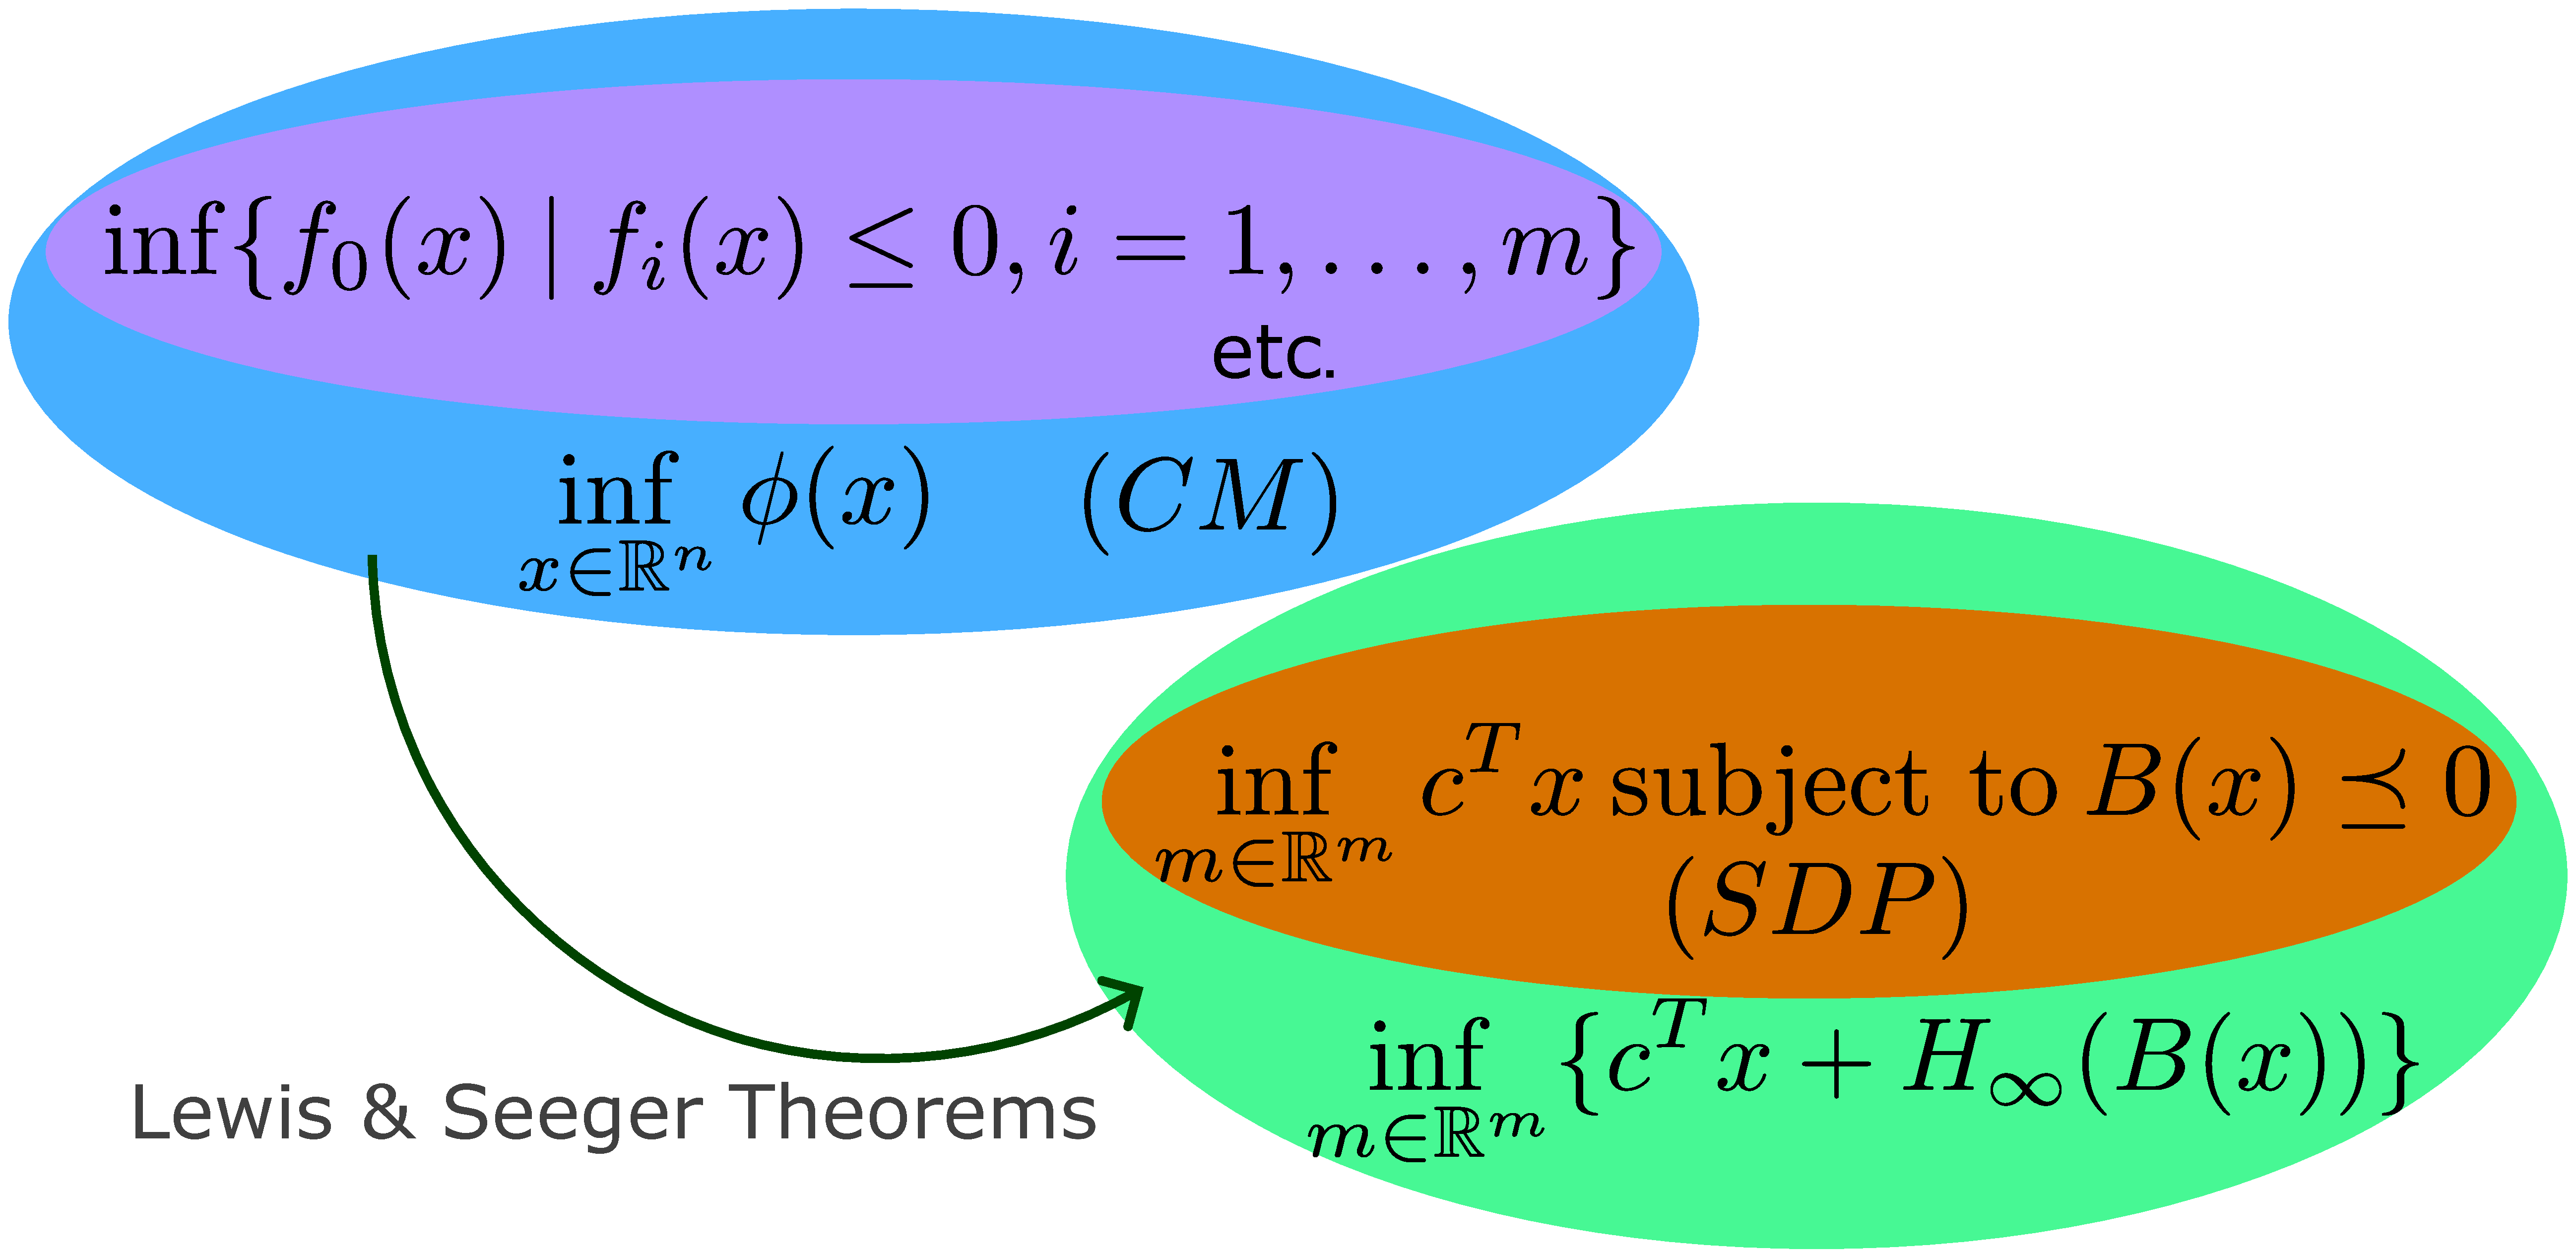
\includegraphics[keepaspectratio, scale=0.105]{figures/summary_of_presentation.eps}
\end{frame}

% 2. Preliminary
% ----------------------------------------------------------------
\section{Preliminary}

% 2.1 Preliminary of symbols like R^n and S^n
\begin{frame}{Preliminary}
$\NDemenstionalRealEuclideanSpace$: $n$-dimensional real Euclidean space. \\
$\NDemenstionalRealSymmetricMatrixSpace$: $n$-dimensional real symmetric matrix space.

The inner product of $\NDemenstionalRealEuclideanSpace$ $\left\langle \cdot ,\cdot \right\rangle$  is defined by

  \begin{equation}
    \InnerProduct{x}{y} \coloneqq \sum_{i = 1}^{n} x_i y_i \:\text{for}\: x=(x_1,\dots,x_n)^T \in \mathbb{R}^n \:\text{and}\: y=(y_1,\dots,y_n)^T \in \mathbb{R}^n. \notag
  \end{equation}

The norm is defined by $\left\lVert x \right\rVert \coloneqq \InnerProduct{x}{x} ^{1/2} $. Like that, we can define the inner product and the norm of $\NDemenstionalRealSymmetricMatrixSpace$.

  \begin{equation}
    \InnerProduct{X}{Y} \coloneqq \Trace{XY} \:\text{for}\: X,Y \in \NDemenstionalRealSymmetricMatrixSpace \quad \text{and} \quad \left\lVert X \right\rVert \coloneqq \InnerProduct{X}{X} ^{1/2} \notag
  \end{equation}
\end{frame}

% 2.2 Preliminary of properties around functions
% domain, epigraph, proper, convex, lsc
\begin{frame}{Preliminary}
  \begin{block}{Definition 1}
    Let $\ExtendedRealValuedFunction{f}{\NDemenstionalRealEuclideanSpace}$.
    \begin{enumerate}
      \item The domain of $f$ is defined by
      \begin{equation}
        \Domain{f} \coloneqq \SetForm{x \in \NDemenstionalRealEuclideanSpace}{f(x) < +\infty}. \notag
      \end{equation}
      \item The epigraph of $f$ is defined by
      \begin{equation}
        \Epigraph{f} \coloneqq \SetForm{(x,y) \in \NDemenstionalRealEuclideanSpace \times \RealNumberSet}{f(x) \leq y}. \notag
      \end{equation}
      \item $f$ is called proper if $\Domain{f} \neq \emptyset$.
      \item $f$ is called convex if $\Epigraph{f}$ is convex.
      \item $f$ is called lower semicontinuous (l.s.c.) if $\Epigraph{f}$ is closed.
    \end{enumerate}
  \end{block}
\end{frame}

% 2.3 Preliminary of properties around functions
% conjugate and symmetric
\begin{frame}{Preliminary}
  \begin{block}{Definition 2}
    Let $\ExtendedRealValuedFunction{f}{\NDemenstionalRealEuclideanSpace}$.
    The conjugate function of $f$ is defined by
    \begin{equation}
      \ConjugateFunction{f}(y) \coloneqq \sup_{x \in \NDemenstionalRealEuclideanSpace} \{ \InnerProduct{x}{y} - f(x) \}. \notag
    \end{equation}
  \end{block}

  \begin{block}{Definition 3}
    Let $\ExtendedRealValuedFunction{f}{\NDemenstionalRealEuclideanSpace}$.
    $f$ is said to be symmetric if
    \begin{equation}
      \forall x \in \NDemenstionalRealEuclideanSpace \:\text{and}\: P: n \times n \text{ permutation matrix}, f(Px) = f(x). \notag
    \end{equation}
  \end{block}
\end{frame}

% 3. Spectrally defined matrix functions
% ----------------------------------------------------------------
\section{Spectrally defined matrix functions}

% 3.1 Definition of Spectrally defined matrix functions
\begin{frame}{Spectrally defined matrix functions}
  \begin{block}{Definition 4}
    The function $\ExtendedRealValuedFunction{\Phi}{\NDemenstionalRealSymmetricMatrixSpace}$ is said to be spectrally defined if there exists a symmetric function $\ExtendedRealValuedFunction{f}{\NDemenstionalRealEuclideanSpace}$ such that
    \begin{equation}
      \Phi (X) = \Phi_{f}(X) \coloneqq f(\lambda (X)), \forall X \in \NDemenstionalRealSymmetricMatrixSpace \notag
    \end{equation}
    where $\lambda (X) \coloneqq (\lambda_1 (X), \dotsb , \lambda_n (X))^T$ is the vector of eigenvalues of $X$ in nondecreasing order.
  \end{block}

  \pause
  \begin{example}
    When we define a symmetric function $f$, a spectrally defined function is deduced:
      \begin{equation}
        f(\lambda)=
          \begin{cases}
            - \Sigma_{i = 1}^{n} \log \lambda_i & \text{\rm if}\:\lambda > 0; \\
            +\infty & \text{\rm otherwise} \notag
          \end{cases} ,\text{\rm and then} \quad
          \Phi_{f}(X)=
          \begin{cases}
            - \log \det (X) & \text{\rm if}\:X \succ 0; \\
            +\infty & \text{\rm otherwise}. \notag
          \end{cases}
      \end{equation}
  \end{example}
\end{frame}

% 3.2 Theorem of Spectrally defined matrix functions and conjugacy
\begin{frame}{Spectrally defined matrix functions}
  \begin{block}{Theorem 5 (A.S.Lewis (1996))}
    Suppose that the function $\ExtendedRealValuedFunction{f}{\NDemenstionalRealEuclideanSpace}$ is symmetric, then
    \begin{equation}
      {\Phi_{f}}^* = \Phi_{f^*} \notag
    \end{equation}
    where ${\Phi_{f}}^* (Y) \coloneqq \sup \{\InnerProduct{X}{Y} - \Phi_{f} (X) \:|\: X \in \NDemenstionalRealSymmetricMatrixSpace\}, \forall Y \in \NDemenstionalRealSymmetricMatrixSpace$.
  \end{block}

  \begin{alertblock}{Remark}
    As a result of Theorem 5, the optimization problems $\min \{\Phi_{f}(X) \:|\: X \in \NDemenstionalRealSymmetricMatrixSpace\}$ and $\min \{f(x) \:|\: x \in \NDemenstionalRealEuclideanSpace\}$ are equivalent. In fact,

    \begin{align}
      \inf_{X \in \NDemenstionalRealSymmetricMatrixSpace} \Phi_{f}(X) &= - \sup_{X \in \NDemenstionalRealSymmetricMatrixSpace} \{- \Phi_{f}(X)\} = - \sup_{X \in \NDemenstionalRealSymmetricMatrixSpace} \{\InnerProduct{X}{0} - \Phi_{f}(X)\} \notag \\
      &= - \Phi^*_{f}(0) = - \Phi_{\ConjugateFunction{f}}(0) = - \ConjugateFunction{f}(0) = \inf_{x \in \NDemenstionalRealEuclideanSpace} f(x). \notag
    \end{align}
  \end{alertblock}
\end{frame}

% 4. Asymptotic cones and functions
% ----------------------------------------------------------------
\section{Asymptotic cones and functions}

% 4.1
\begin{frame}{What is the notion of asymptotic cones?}
  \pause
  $\rightarrow$ To look at something from a distance, that is, to zoom out.

  \medskip

  \centering
    \begin{columns}
      \pause
      \begin{column}{0.48\textwidth}
      \centering
      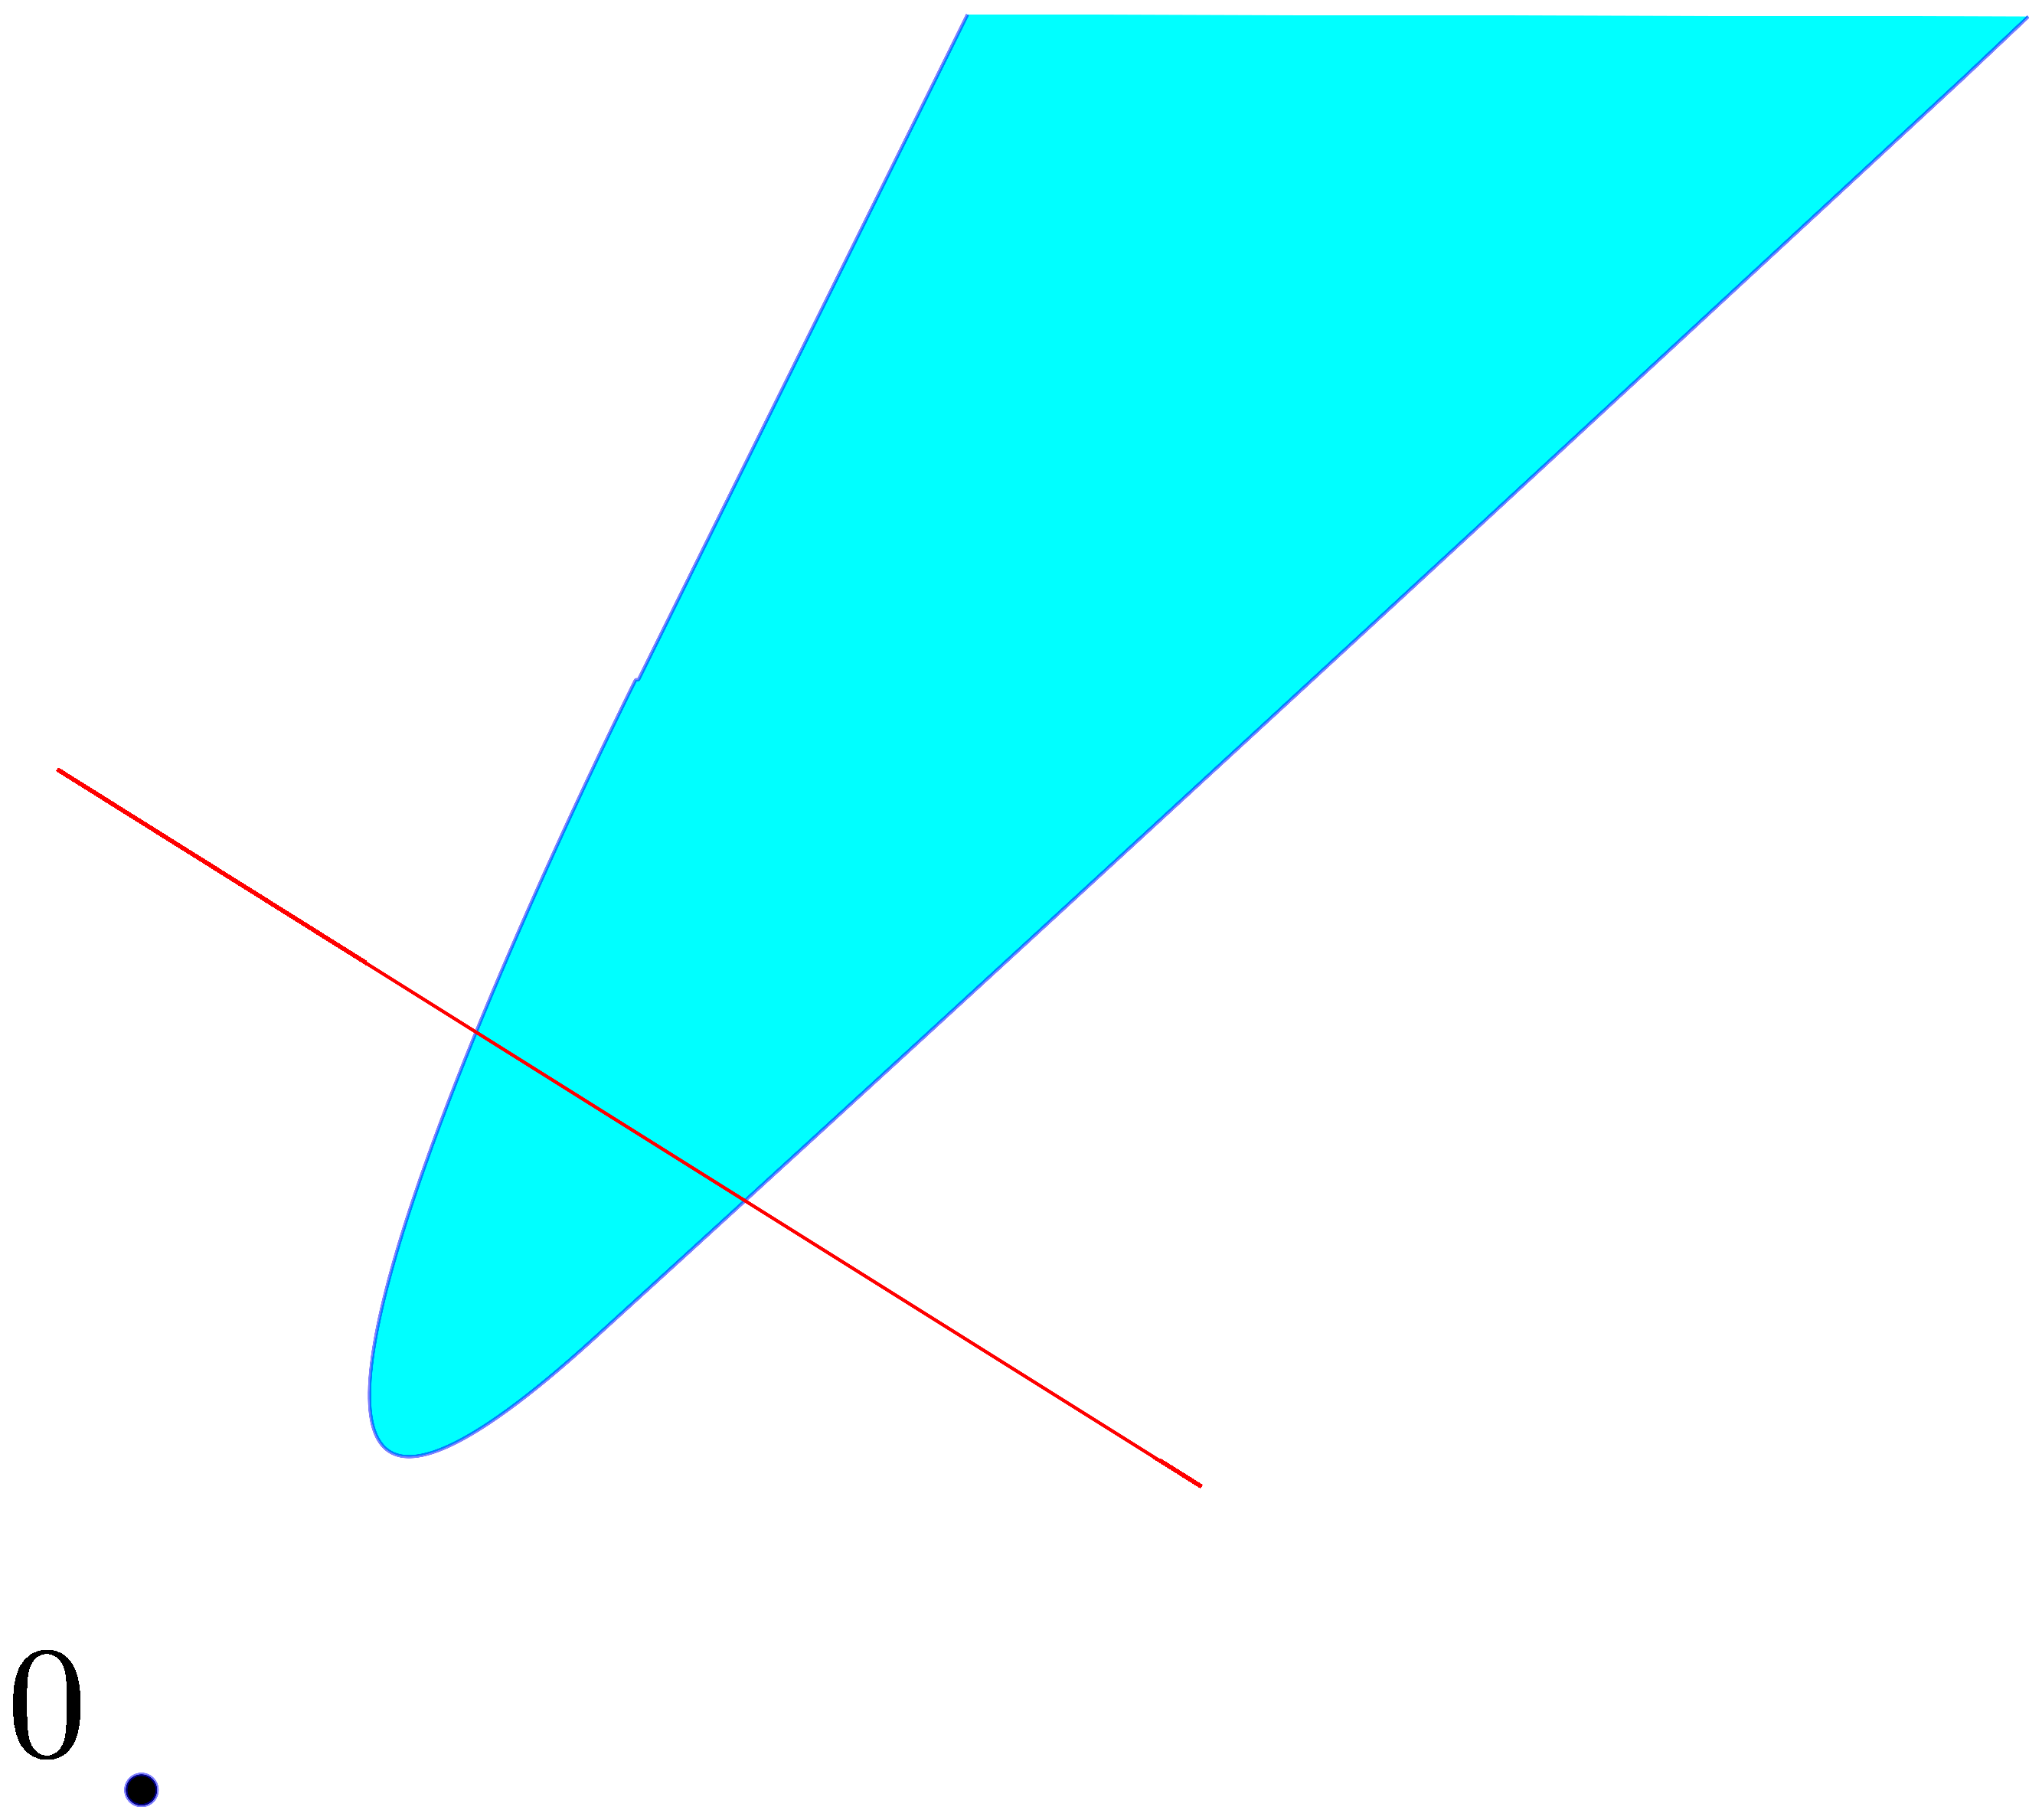
\includegraphics[keepaspectratio, scale=0.095]{figures/asymptotic_meaning_1.eps}
      \end{column}
      \pause
      \begin{column}{0.48\textwidth}
      \centering
      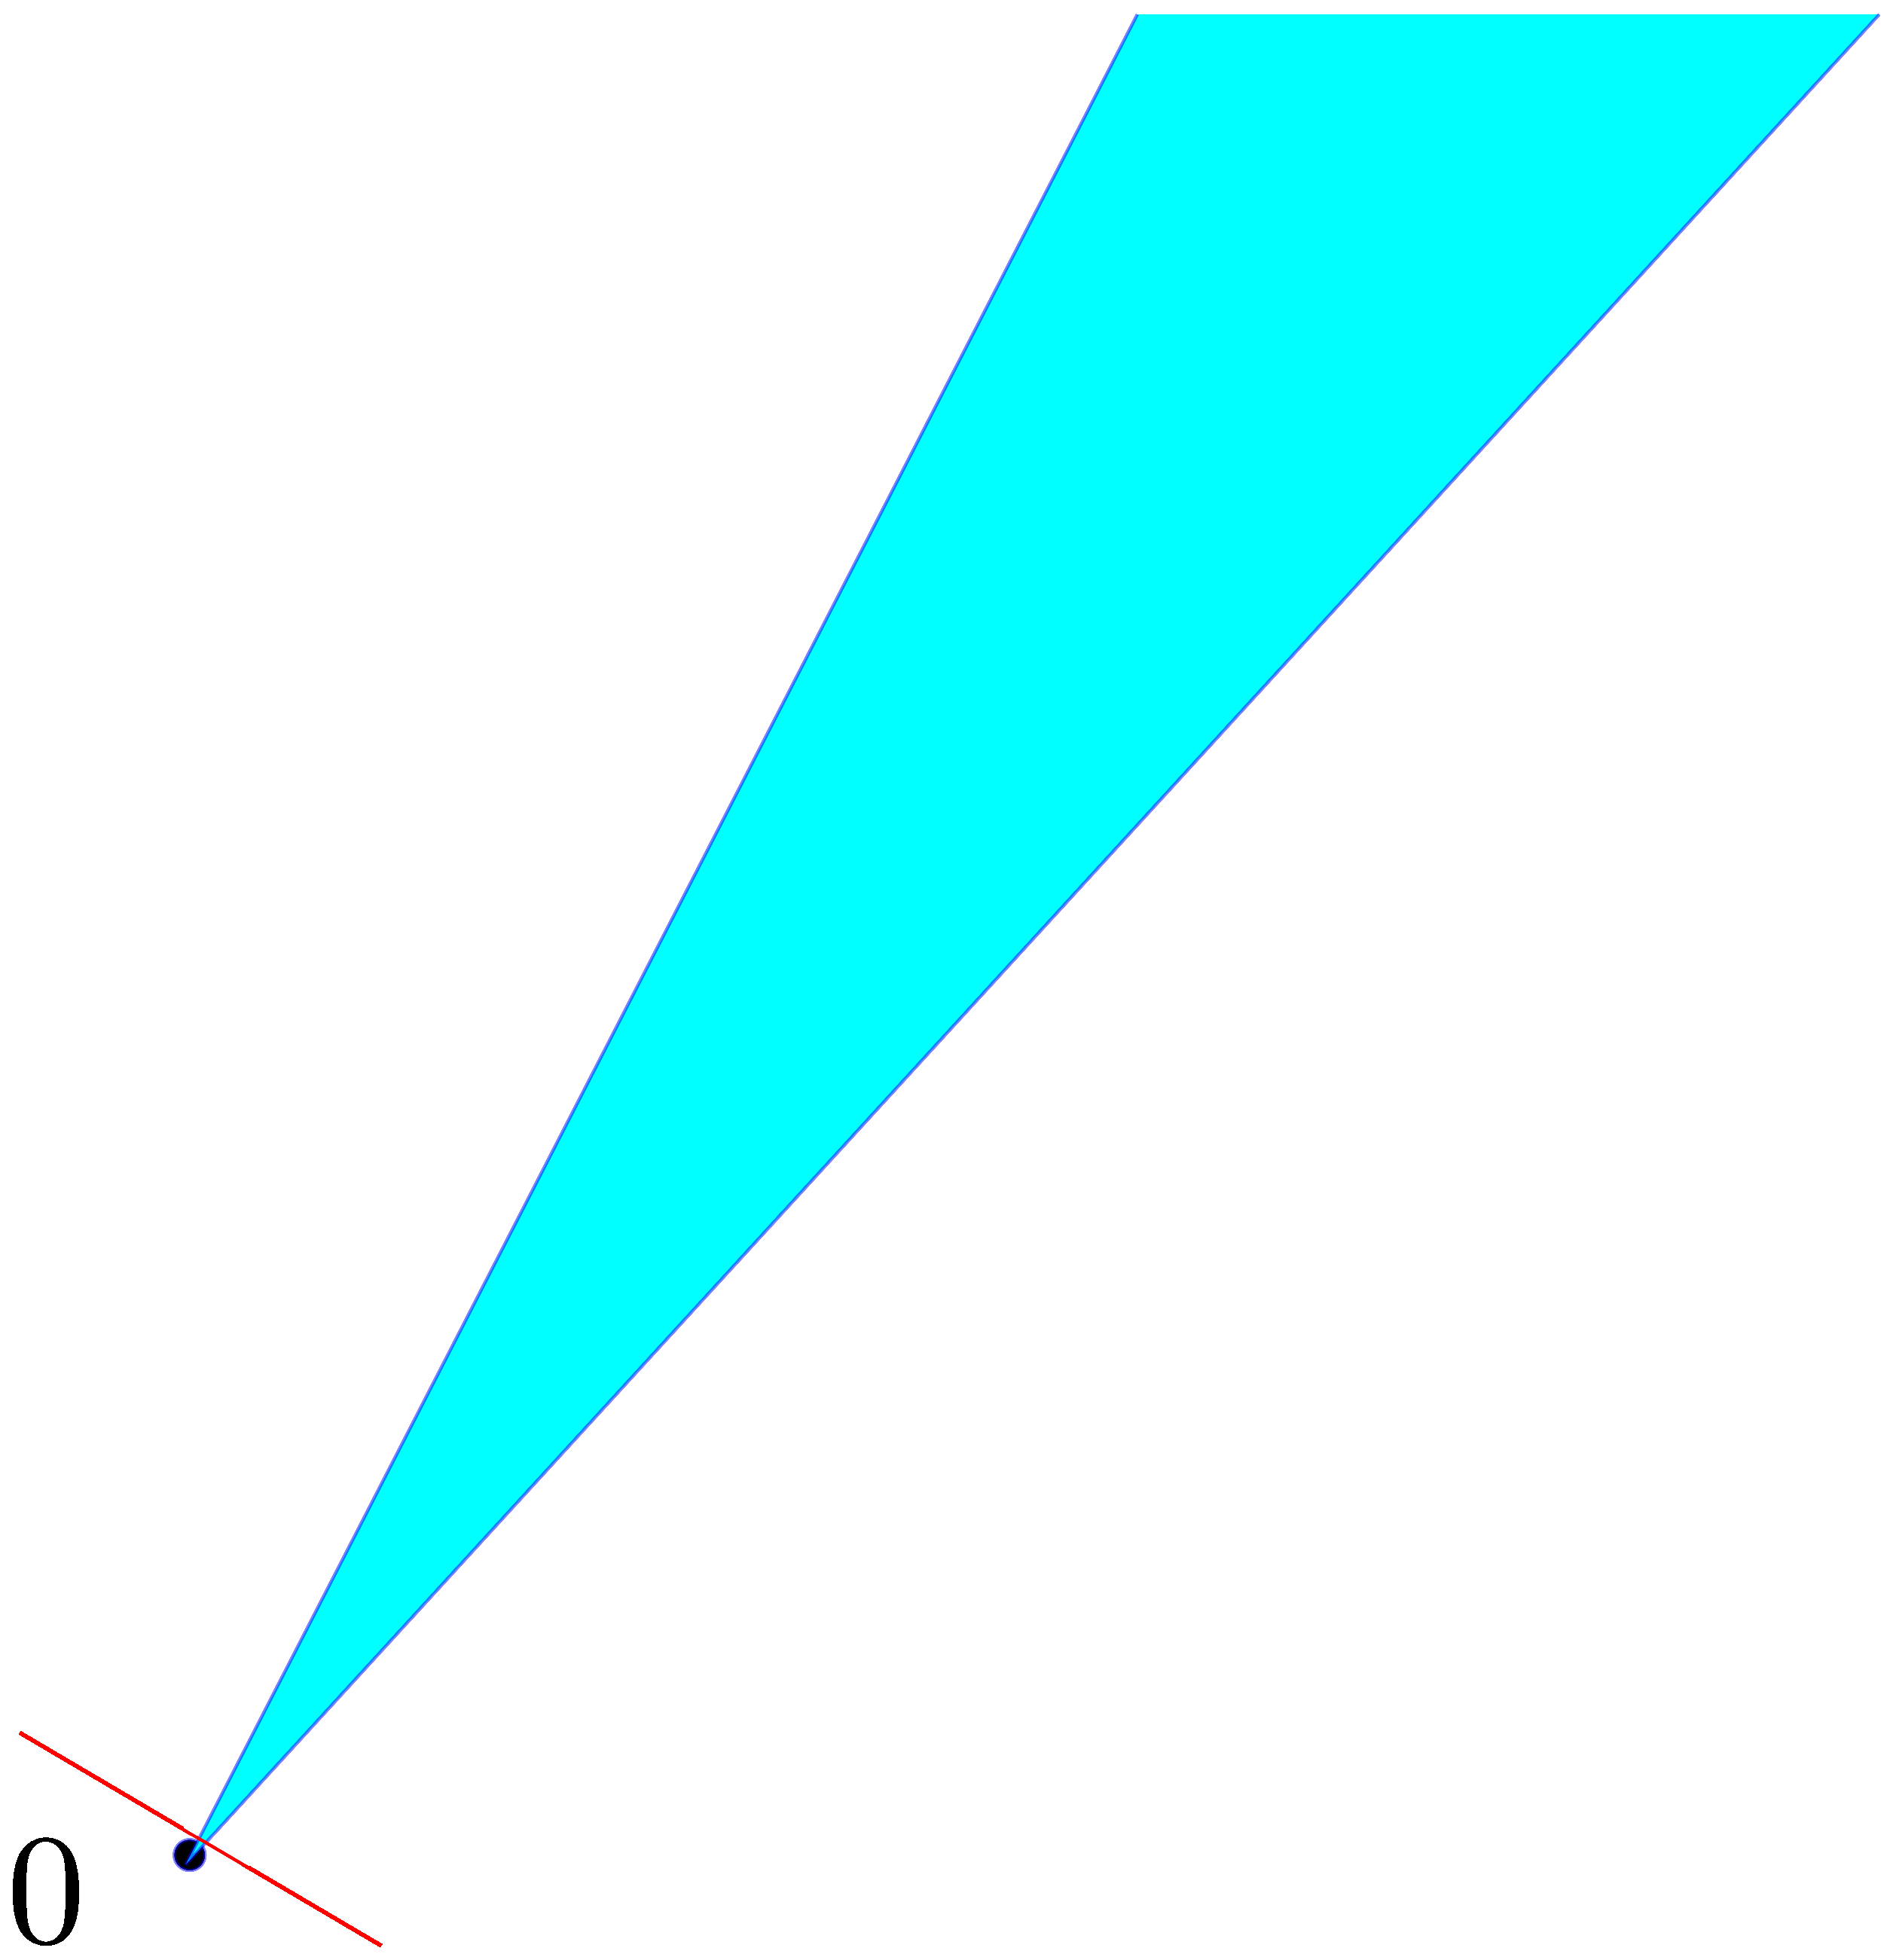
\includegraphics[keepaspectratio, scale=0.095]{figures/asymptotic_meaning_2.eps}
    \end{column}
  \end{columns}
\end{frame}

% 4.2
\begin{frame}{Definition of Asymptotic Cones}
  \begin{block}{Definition 6}
    $C \subset \mathbb{R}^n$, $C \neq \emptyset$. Then, the asymptotic cone of the set $C$, denoted by $C_\infty$, is the set below with $\{ x_k \} \subset C$;
    \begin{equation}
      C_\infty = \left\{ d \in
      \mathbb{R}^n \:\middle|\: \exists t_k \rightarrow +\infty, \exists x_k \in C \:\text{\rm with}\: \lim_{k \to \infty} \frac{x_k}{t_k} = d \right\}. \notag
    \end{equation}
  \end{block}

  Example: $C = \{(x,y) \in \mathbb{R}^2 \:|\: y=x^2\}$. We let $\textcolor{blue}{x_k} = (k, k^2)$ and $t_k = \left\lVert x_k \right\rVert$.

  \centering
  \begin{columns}
    \pause
    \begin{column}{0.48\textwidth}
    \centering
    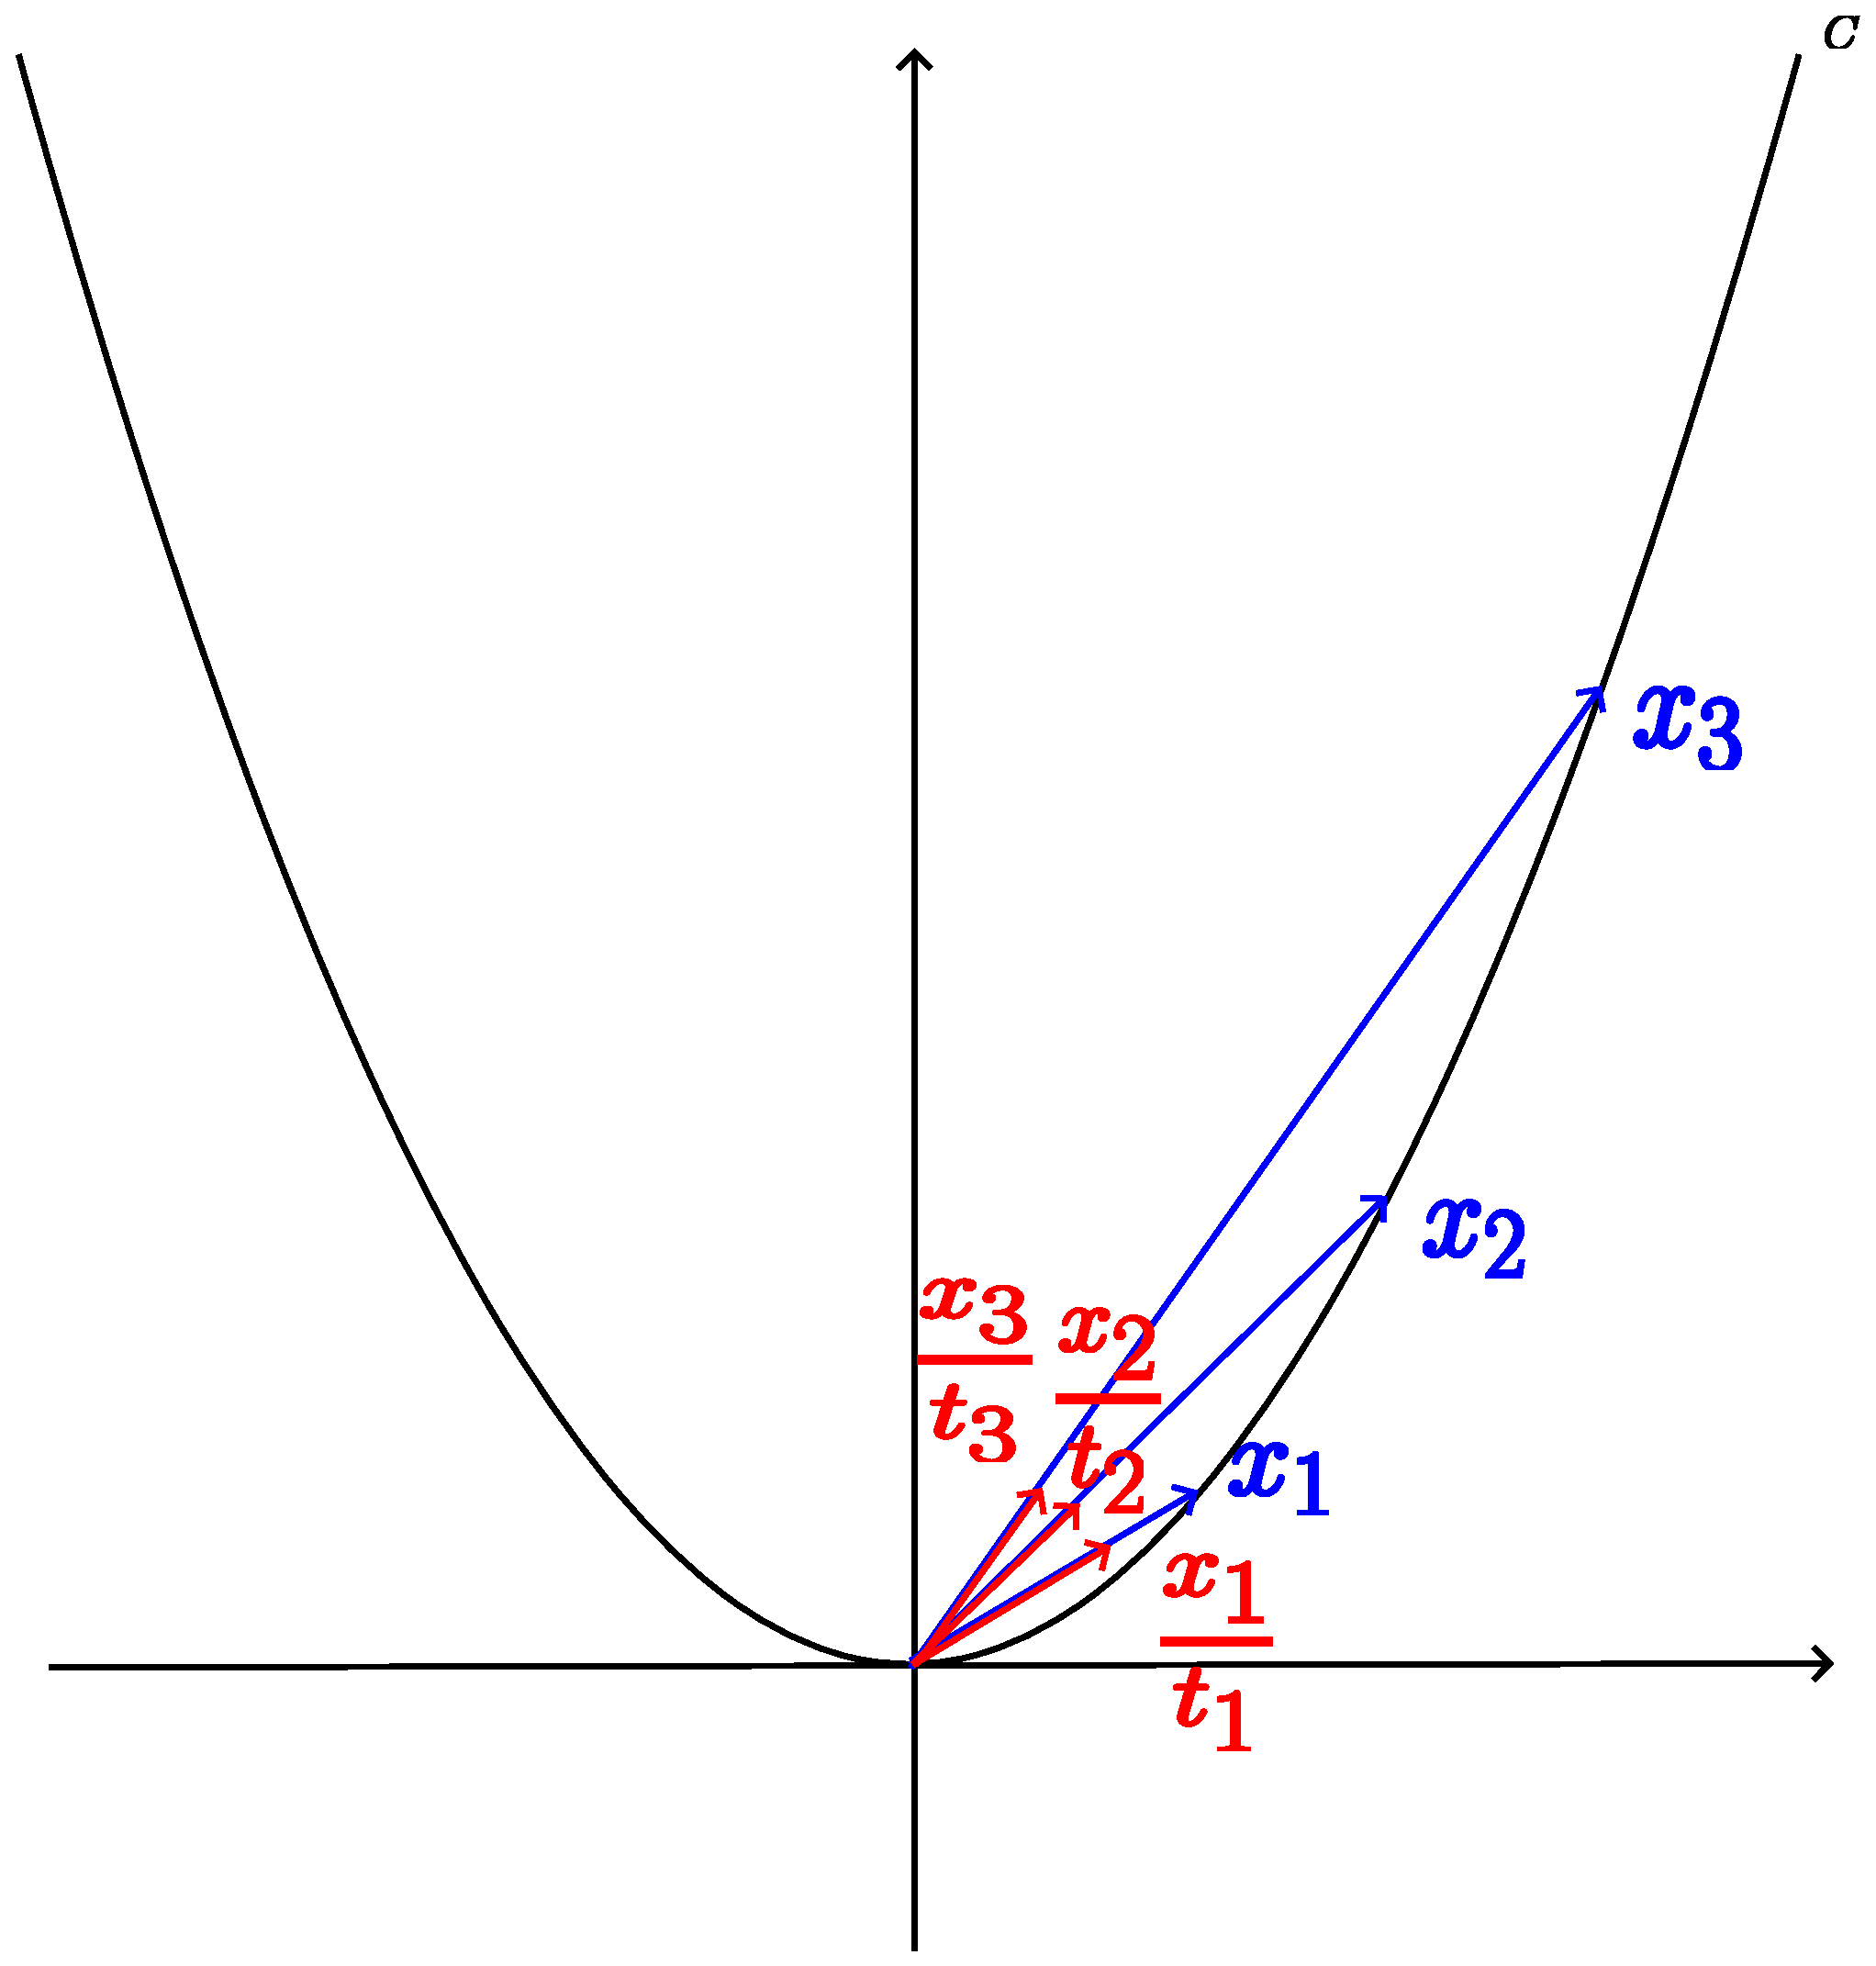
\includegraphics[keepaspectratio, scale=0.09]{figures/figure_asymptotic_cone_1.eps}
    \end{column}
    \pause
    \begin{column}{0.48\textwidth}
    \centering
    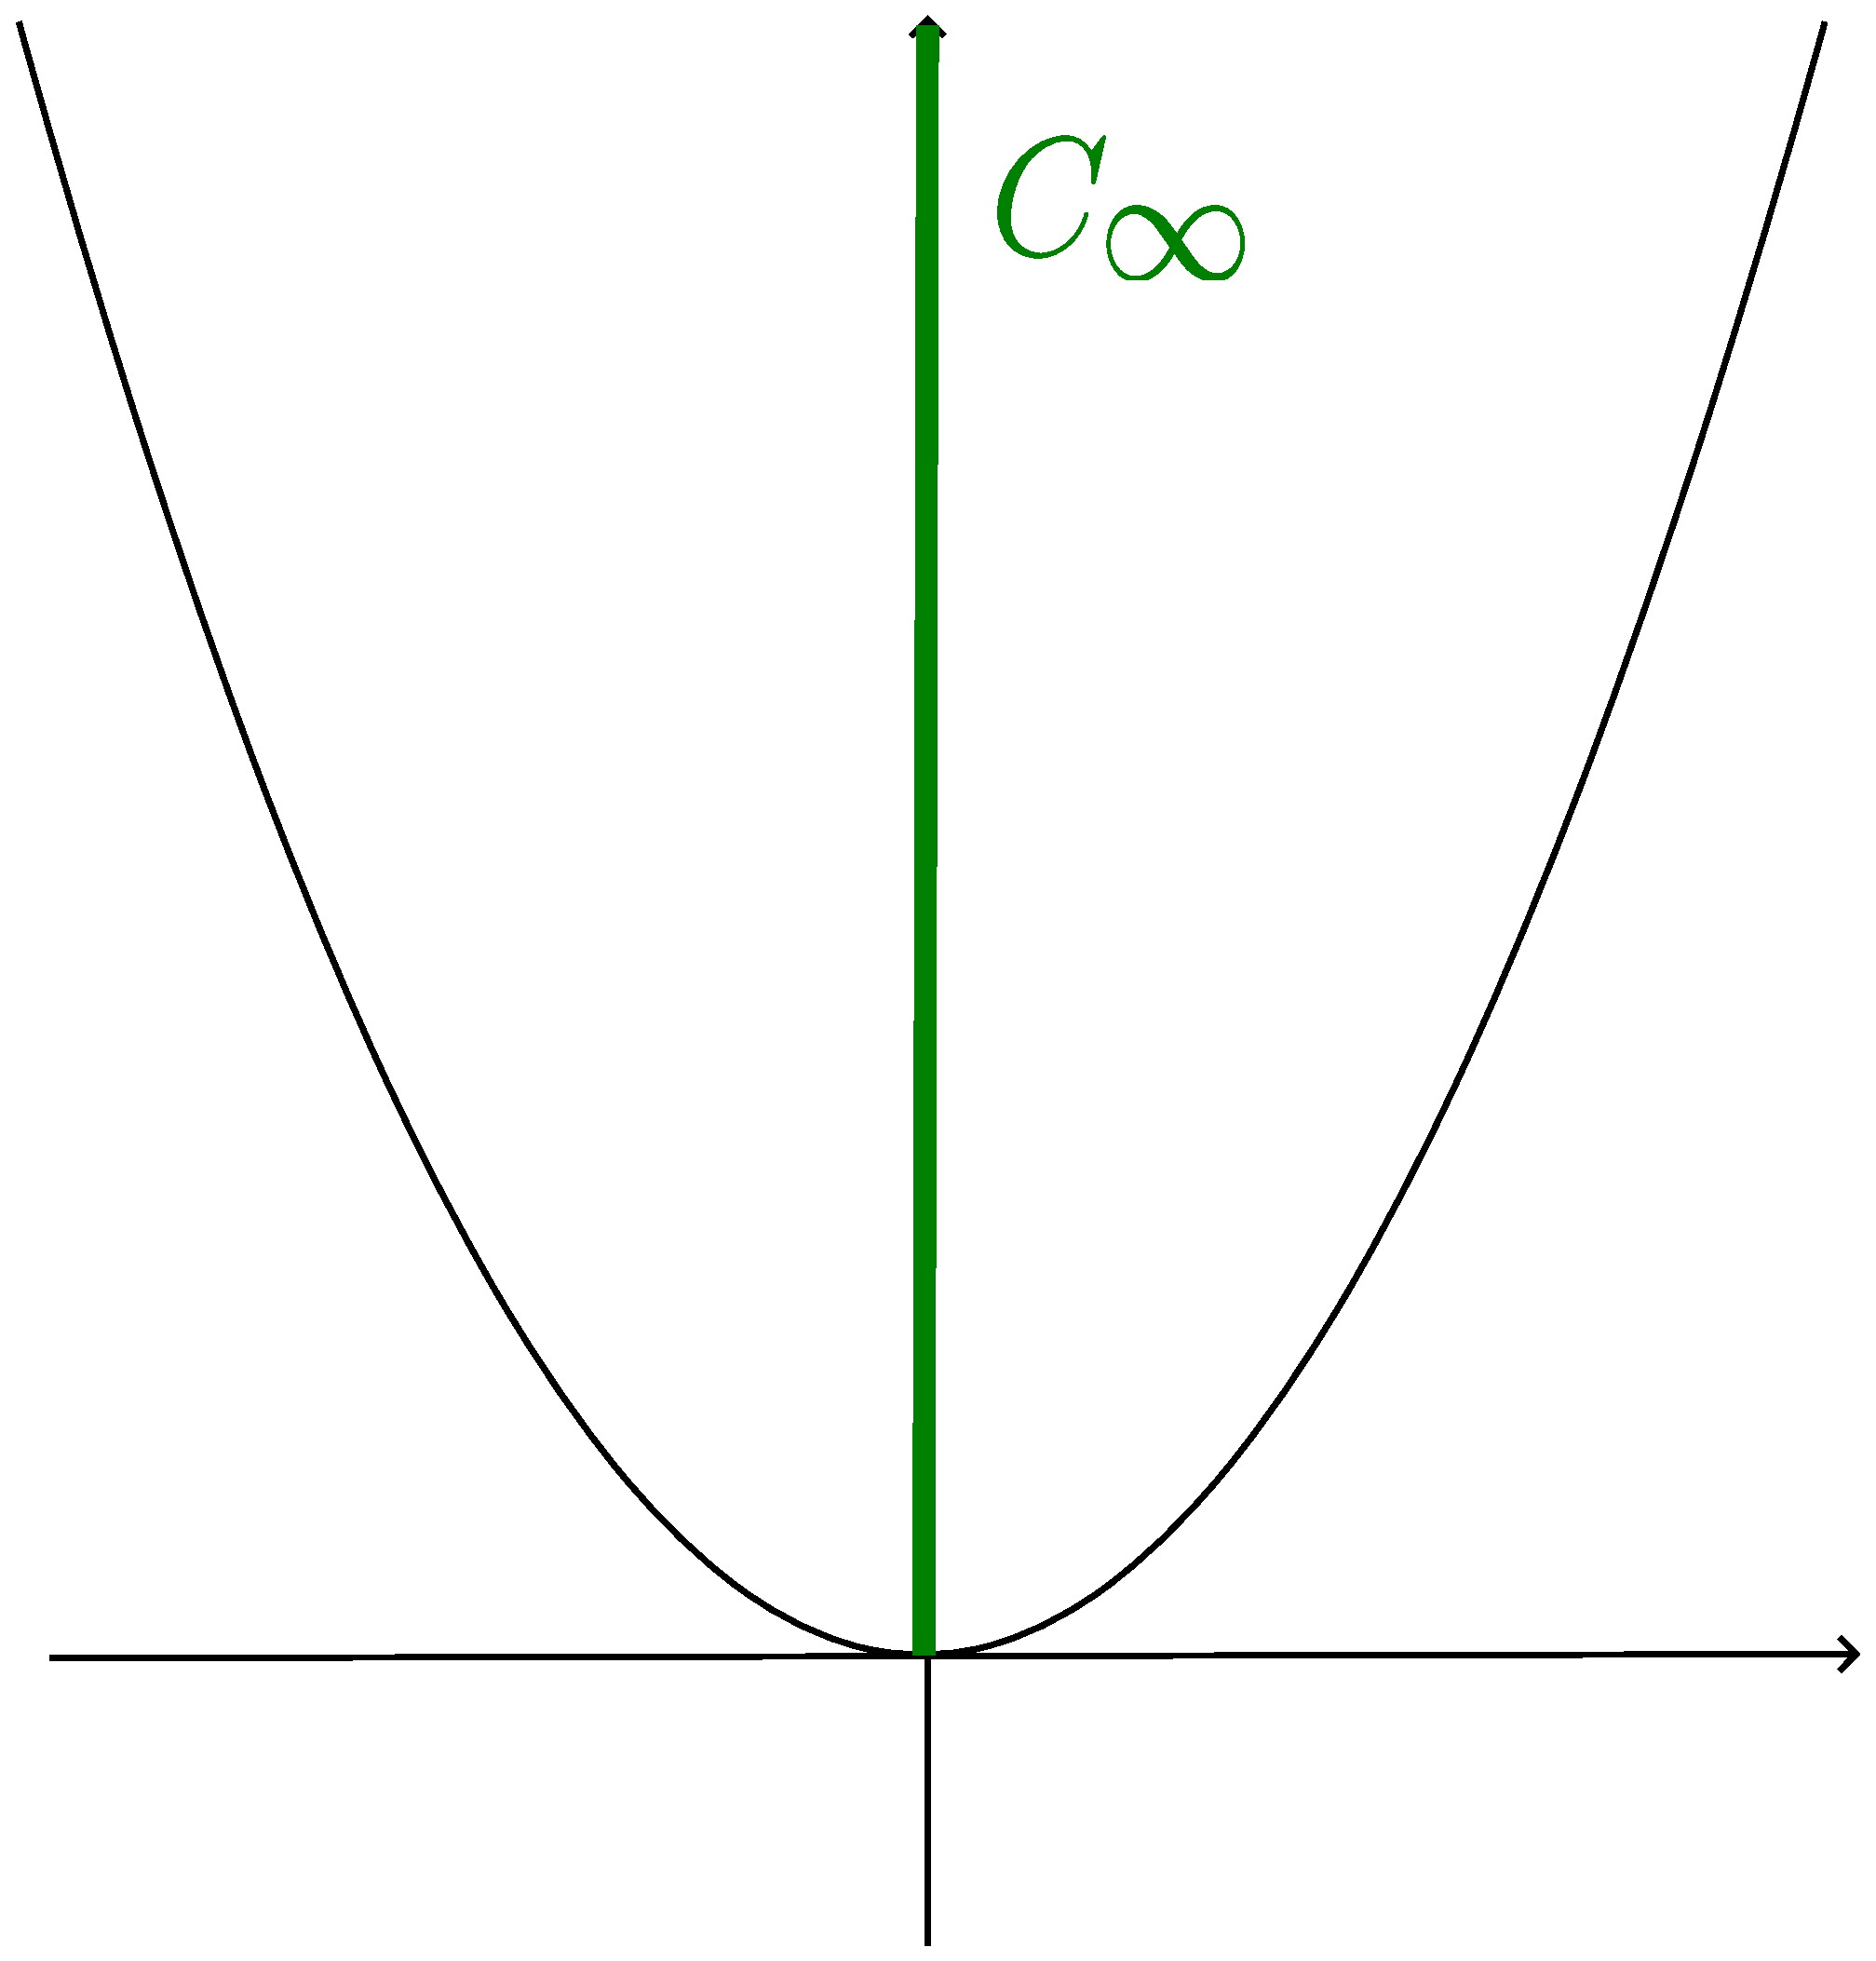
\includegraphics[keepaspectratio, scale=0.09]{figures/figure_asymptotic_cone_2.eps}
    \end{column}
  \end{columns}
\end{frame}

% 4.3
\begin{frame}{Properties around Asymptotic Cones}
  \begin{block}{Proposition 7}
    Let $C$ be a nonempty convex set in $\NDemenstionalRealEuclideanSpace$. Then the asymptotic cone $C_{\infty}$ is a closed convex cone. Moreover, define the following sets;
    \begin{align}
      D(x) &\coloneqq \SetForm{d \in \NDemenstionalRealEuclideanSpace}{x+td \in \Closure{C}, \forall t > 0} \forall x \in C, \notag \\
      E &\coloneqq \SetForm{d \in \NDemenstionalRealEuclideanSpace}{\exists x \in C \SuchThat x+td \in \Closure{C}, \forall t > 0}, \notag \\
      F &\coloneqq \SetForm{d \in \NDemenstionalRealEuclideanSpace}{d + \Closure{C} \subset \Closure{C}}. \notag
    \end{align}
    Then $D(x)$ is in fact independent of $x$, which is thus now denoted by $D$, and $C_{\infty} = D = E = F$.
  \end{block}

  \begin{alertblock}{Remark}
    When $C$ is a closed convex set, the asymptotic cone is also called the recession cone. In this presentation, we use the term the asymptotic cone.
  \end{alertblock}
\end{frame}

% 4.4
\begin{frame}{Definition of Asymptotic Functions}
  \begin{block}{Definition 8}
    Let $f: \NDemenstionalRealEuclideanSpace \rightarrow \RealNumberSet \cup \{+\infty\}$ be proper. Then, there exists $f_{\infty}: \NDemenstionalRealEuclideanSpace \rightarrow \RealNumberSet \cup \{\pm\infty\}$ satisfying $\Epigraph{f_{\infty}} = (\Epigraph{f})_{\infty}$, which is called asymptotic function of $f$.
  \end{block}

  \pause
  \begin{exampleblock}{How to create asymptotic function of $f$}
    To gain asymptotic function of $f$, we have 4 steps including providing the definition of $f$.
    \begin{enumerate}
      \item provide $f$
      \item consider $\Epigraph{f}$
      \item take $(\Epigraph{f})_{\infty}$, the asymptotic cone of $(\Epigraph{f})$
      \item define $f_{\infty}$
    \end{enumerate}
  \end{exampleblock}
\end{frame}

% 4.5
\begin{frame}{How to create Asymptotic Functions}
  \begin{figure}[htbp]
    \begin{tabular}{cc}
      \begin{minipage}[t]{0.45\hsize}
        \centering
        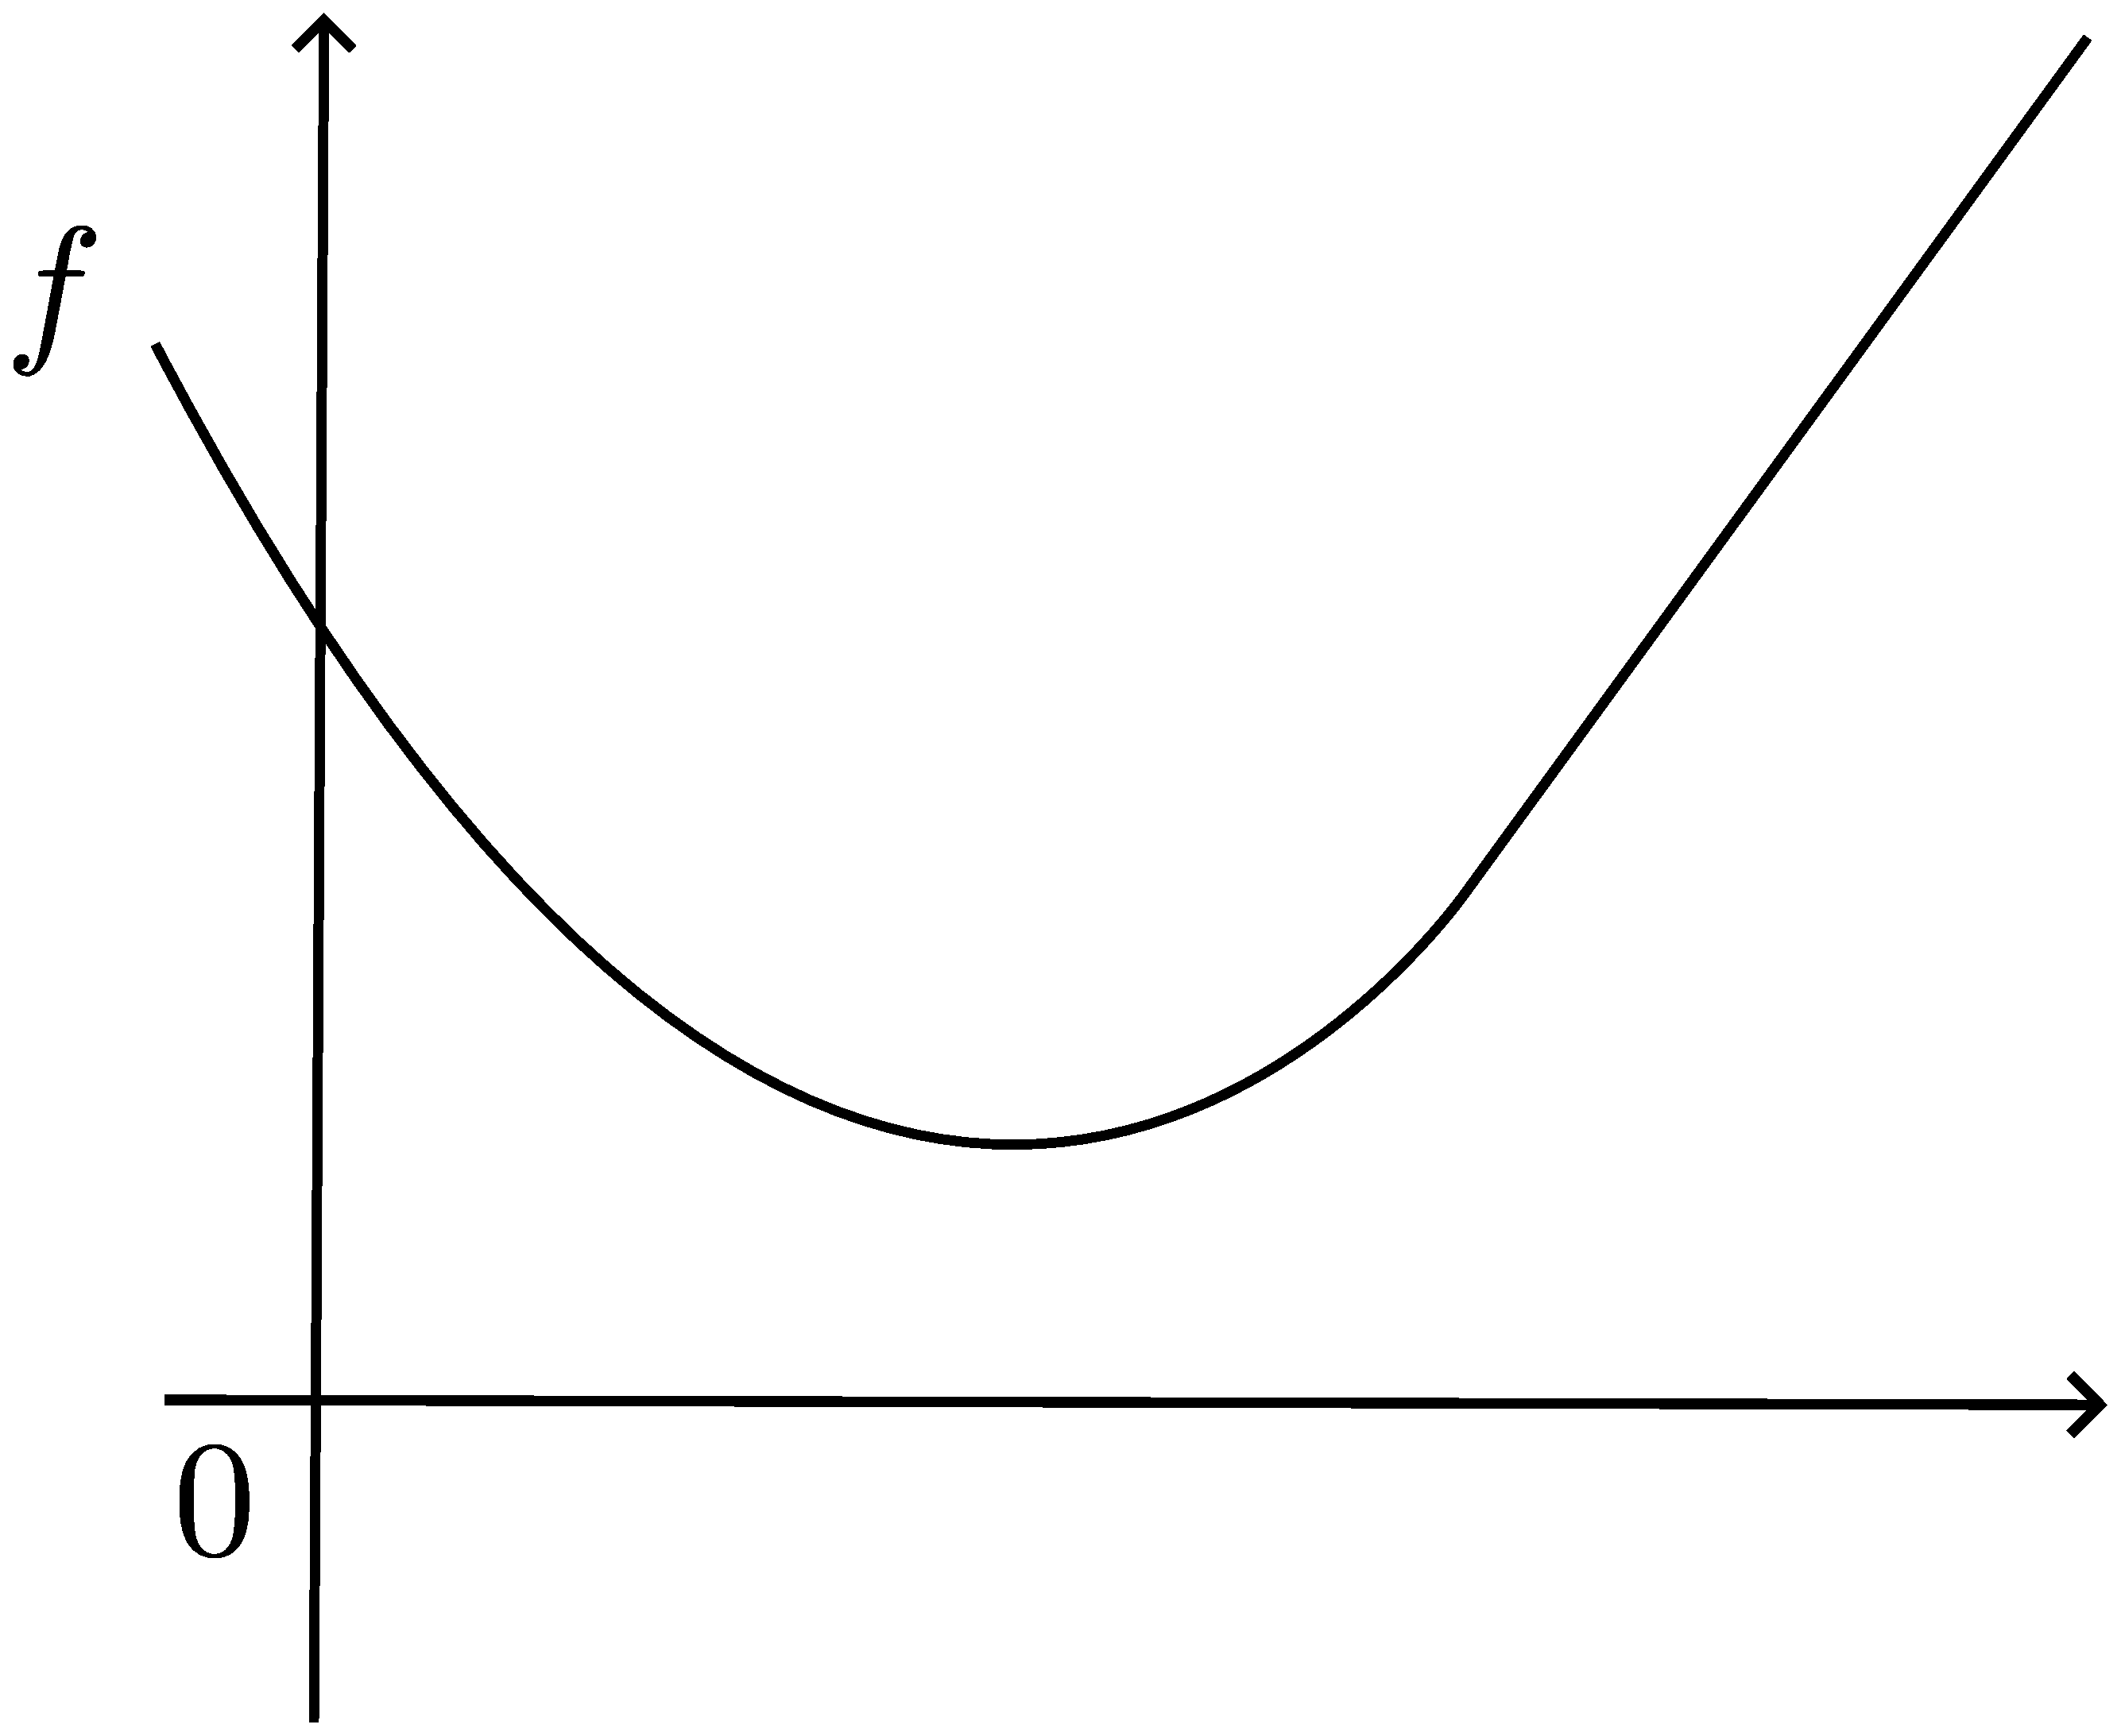
\includegraphics[keepaspectratio, scale=0.06]{figures/asymptotic_function_def/graph_base.eps}
        \caption{(1) provide $f$}
      \end{minipage} &
      \begin{minipage}[t]{0.45\hsize}
        \centering
        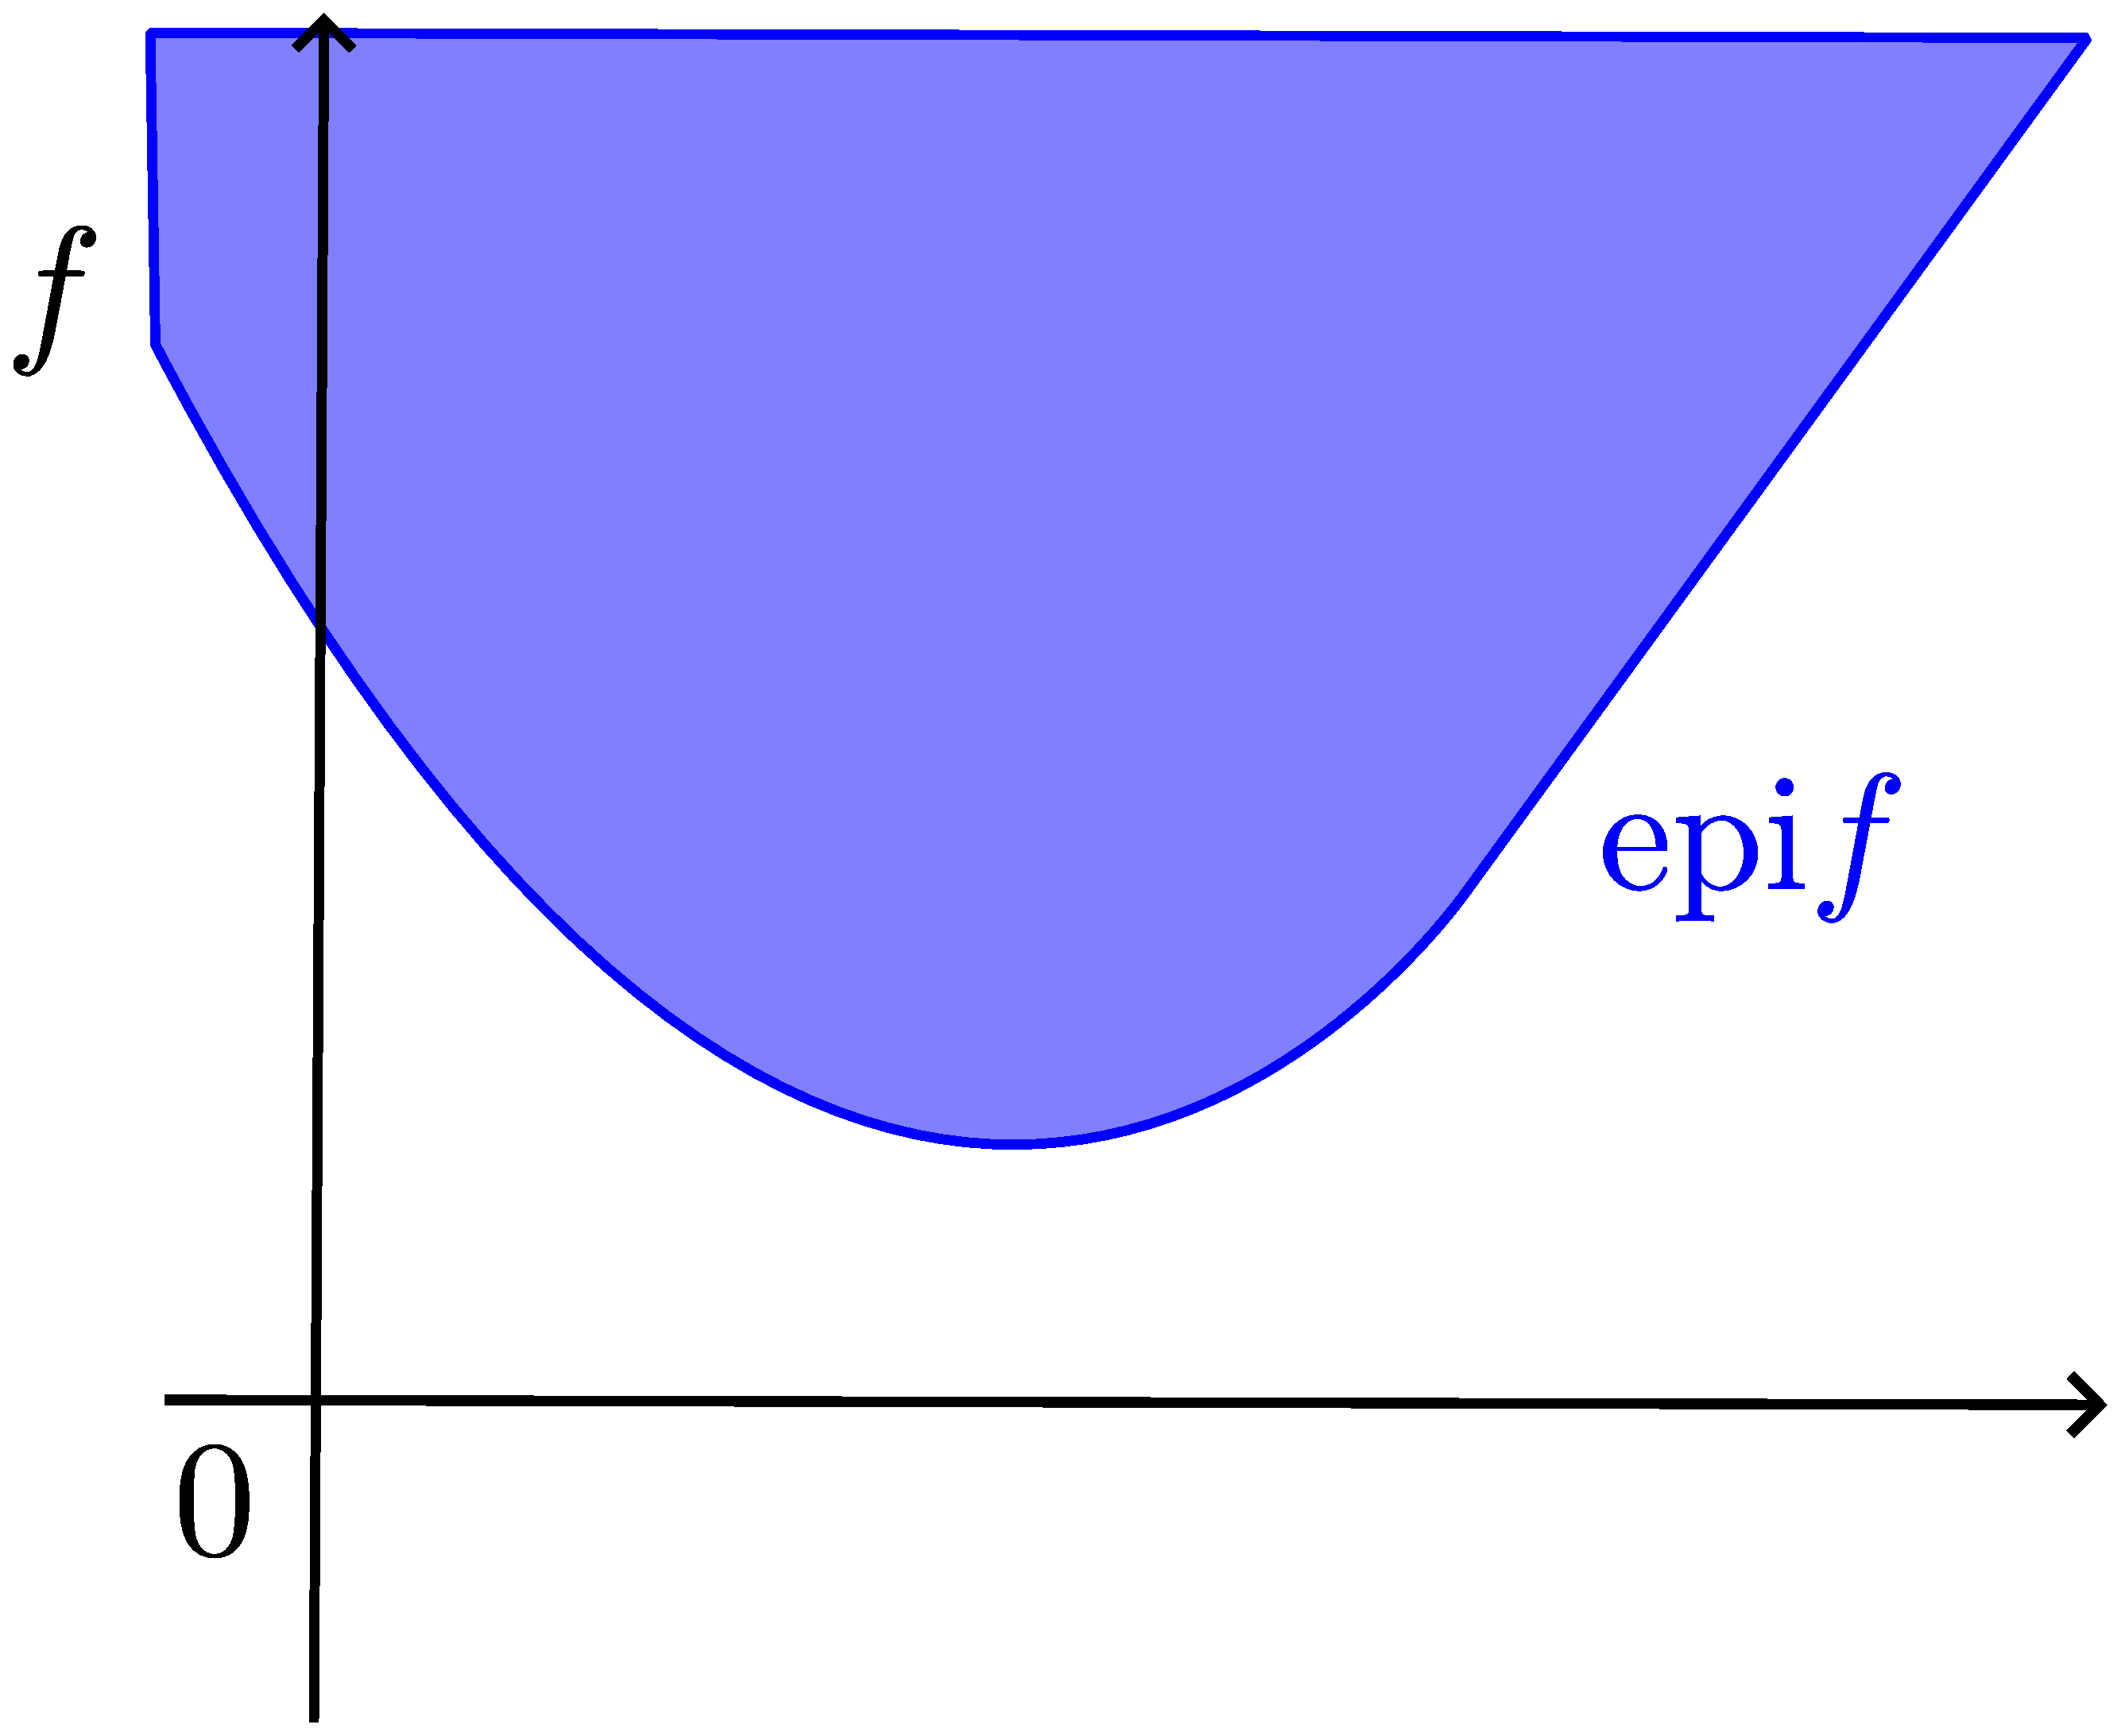
\includegraphics[keepaspectratio, scale=0.06]{figures/asymptotic_function_def/asymptotic_function_epigraph.eps}
        \caption{(2) consider $\Epigraph{f}$}
      \end{minipage} \\

      \begin{minipage}[t]{0.45\hsize}
        \centering
        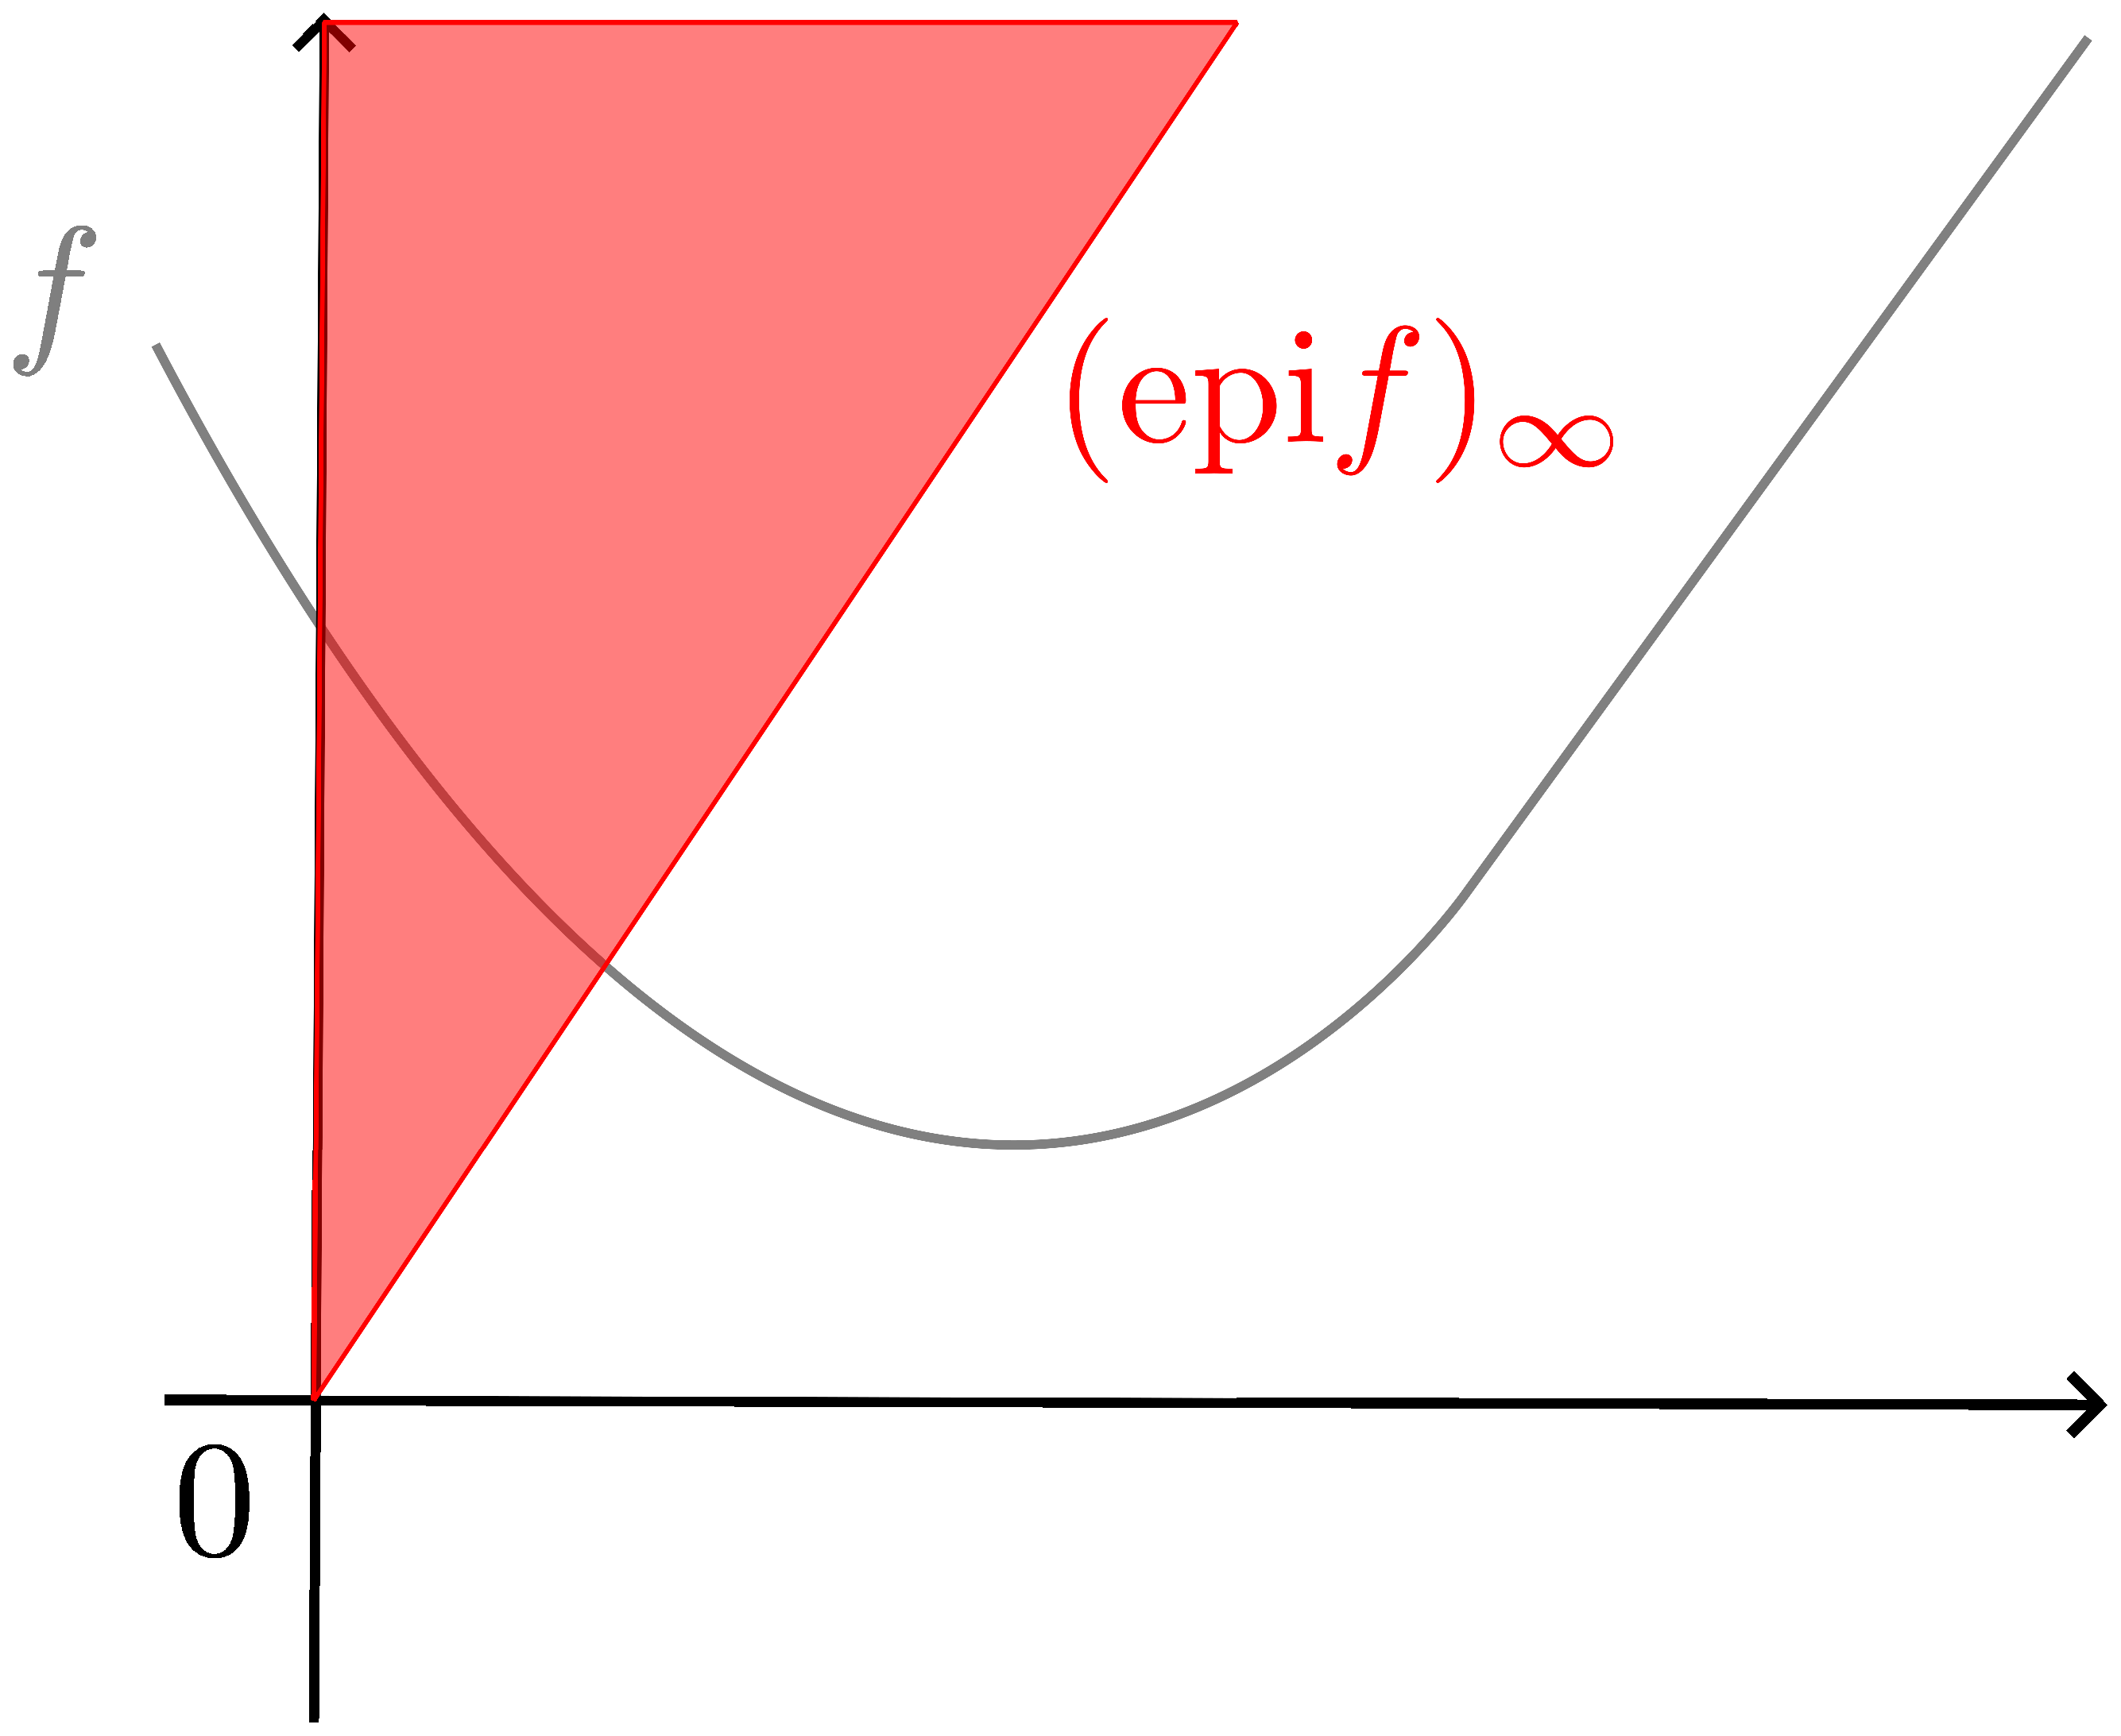
\includegraphics[keepaspectratio, scale=0.06]{figures/asymptotic_function_def/asymptotic_cone_epigraph_f.eps}
        \caption{(3) take the asymptotic cone of $(\Epigraph{f})$}
      \end{minipage} &
      \begin{minipage}[t]{0.45\hsize}
        \centering
        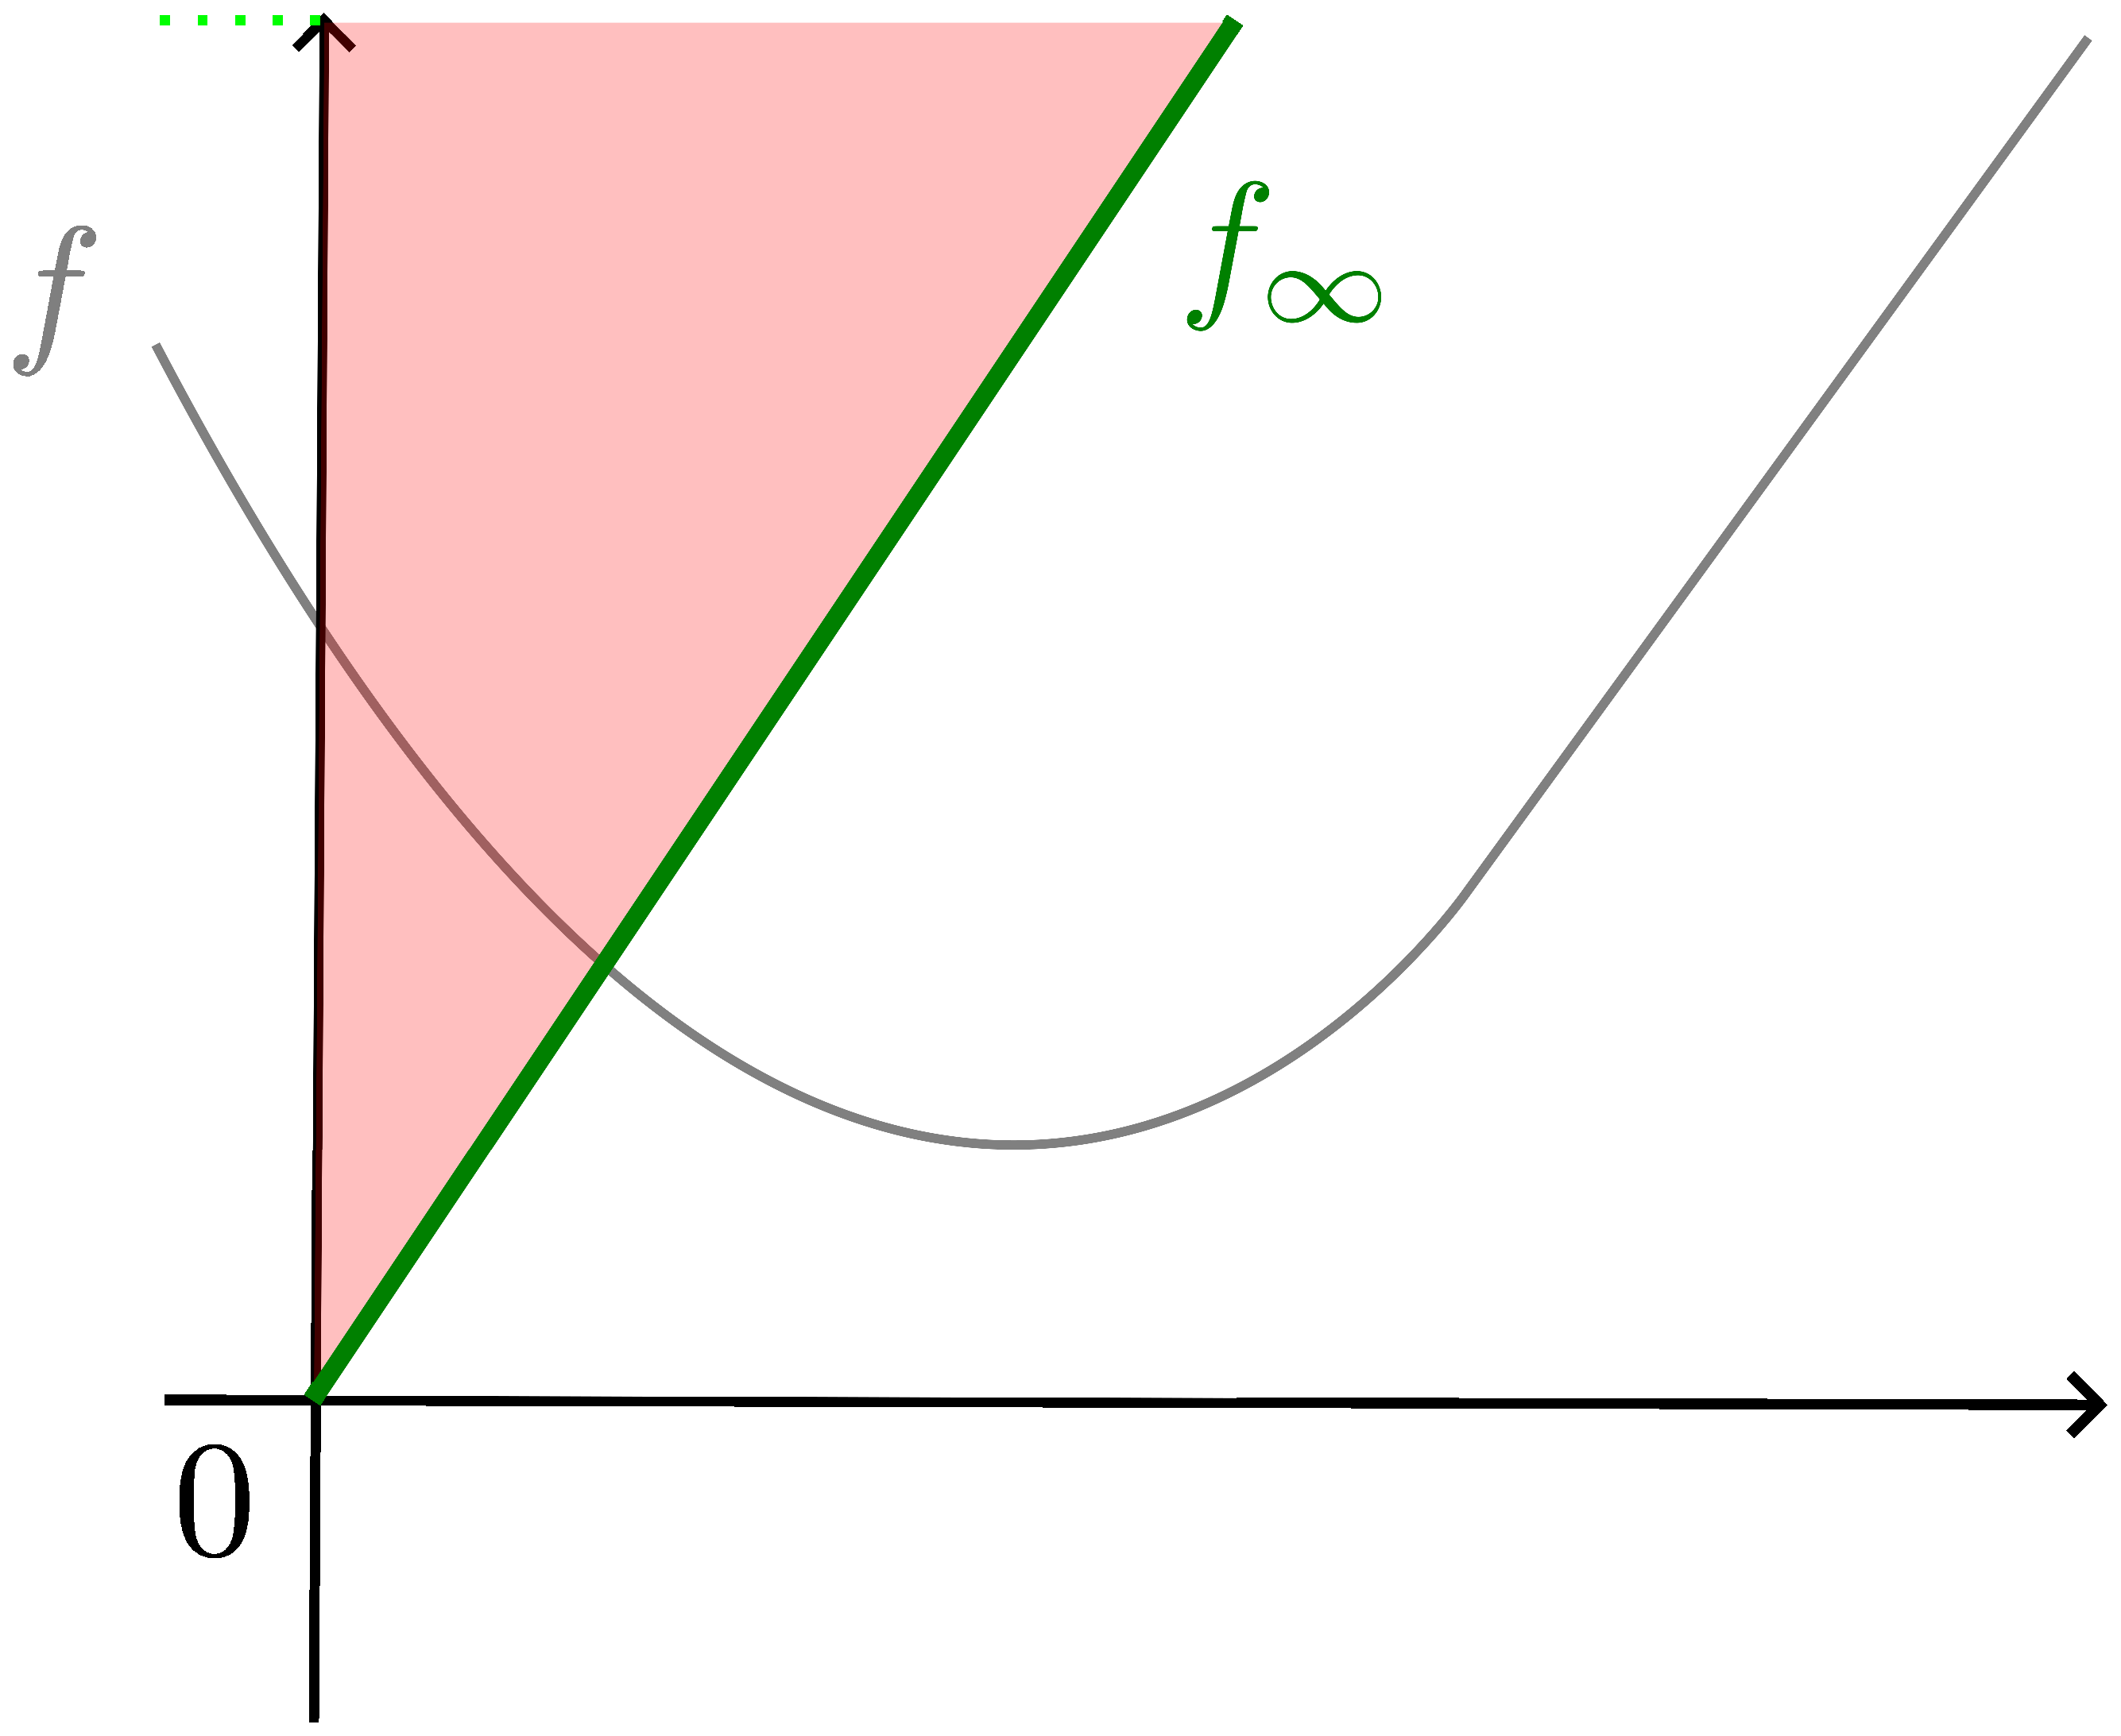
\includegraphics[keepaspectratio, scale=0.06]{figures/asymptotic_function_def/asymptotic_function_f.eps}
        \caption{(4) obtain $f_{\infty}$}
      \end{minipage}
    \end{tabular}
  \end{figure}
\end{frame}

% 4.6
\begin{frame}{Properties around Asymptotic Functions}
  \begin{block}{Proposition 9}
    Let $\ExtendedRealValuedFunction{f}{\NDemenstionalRealEuclideanSpace}$ be a proper, lsc, convex function. Then, the asymptotic function is a lsc, proper, convex function, and one has
    \begin{equation}
      f_{\infty} (d) = \lim_{t \to +\infty} \frac{f(x+td) -f(x)}{t} = \sup_{t > 0} \frac{f(x+td) -f(x)}{t}, \forall x \in \Domain{f} \notag
    \end{equation}
    and
    \begin{equation}
      f_{\infty} (d) = \sup \{\InnerProduct{x}{d} \:|\: x \in \Domain{\ConjugateFunction{f}}\}. \notag
    \end{equation}
  \end{block}
\end{frame}

% 5. Applications of asymptotic functions to SDP
% ----------------------------------------------------------------
\section{Applications of asymptotic functions to SDP}

% 5.1
\begin{frame}{Application of the notion of asymptotic function}
  \begin{block}{Definition 10}
    Following Proposition 9, the asymptotic functions of the proper convex lsc function $\ExtendedRealValuedFunction{\Phi}{\NDemenstionalRealSymmetricMatrixSpace}$ is defined by, for all $D \in \NDemenstionalRealSymmetricMatrixSpace$
    \begin{equation}
      \Phi_{\infty} (D) = \sup_{t > 0} \frac{\Phi(A+tD) -\Phi(A)}{t}, \forall A \in \Domain{\Phi} \quad \text{and}\notag
    \end{equation}
    \begin{equation}
      \Phi_{\infty} (D) = \sup \{\InnerProduct{B}{D} \:|\: B \in \Domain{\ConjugateFunction{\Phi}}\}. \notag
    \end{equation}
  \end{block}

  \begin{block}{Theorem 11 (A.Seeger (1997))}
    Let $\ExtendedRealValuedFunction{f}{\NDemenstionalRealEuclideanSpace}$ be a symmetric, lsc, proper, convex function with induced spectral function $\Phi_{f}$. Then
    \begin{equation}
      {(\Phi_{f})}_{\infty} = \Phi_{f_{\infty}}. \notag
    \end{equation}
  \end{block}
\end{frame}


% 6. Conclusions
% ----------------------------------------------------------------
\section{Conclusion}

% 6.1
\begin{frame}{Conclusion}
  Summary:
  \begin{enumerate}[]
    \item We figure out why a semidefinite programming with a penalty function like log barrier functions can be solved with using Fenchel duality.
    \item Asymptotic function can be applied to spectrally defined functions.
  \end{enumerate}
  Issue:
  \begin{enumerate}[]
    \item These consequences hardly appears in current studies because the way with using barrier function might not be utilized to obtain an optimal value.
    \item Actually, there are strong relations between spectral functions and composite optimization models.
  \end{enumerate}
\end{frame}

% References
% ----------------------------------------------------------------
\begin{frame}[t]{References}
  \begin{enumerate}[]
    \item A. Auslender and M. Teboulle, asymptotic cones and functions in optimization and variational inequalities, Springer monographs in Mathematics, Springer-Verlag, New York, 2003.
    \item A.S. Lewis. Convex Analysis on the Hermitian matrices. SIAM J. Optimization,6, 1996, 164-177.
    \item A. Seeger. Convex analysis of spectrally defined matrix functions. SIAM J. Optimization , 7, 1997, 679-696.
  \end{enumerate}
\end{frame}
\end{document}
